%%%
%% Charles' Hack
%% allow line breaks after hyphens in urls
\PassOptionsToPackage{hyphens}{url}

% openany - Dont foce chapters to start on on right hand page
% oneside - put all page numbers in the upper right, not outer corner
\documentclass[openany, oneside]{tufte-book} 

\hypersetup{colorlinks} % uncomment this line if you prefer colored hyperlinks (e.g., for onscreen viewing)

%%
% Book metadata
\title{Hypercompression}
\author{Charles Holbrow}
%\publisher{Publisher of This Book}

%%
% If they're installed, use Bergamo and Chantilly from www.fontsite.com.
% They're clones of Bembo and Gill Sans, respectively.
%\IfFileExists{bergamo.sty}{\usepackage[osf]{bergamo}}{}% Bembo
%\IfFileExists{chantill.sty}{\usepackage{chantill}}{}% Gill Sans

%\usepackage{microtype}

%%
% Symbol for Euro Currency
\usepackage[official]{eurosym}

%%
% Degree symbol \degree
\usepackage{gensymb}

%%
% For nicely typeset tabular material
\usepackage{booktabs}

%%
% For graphics / images
\usepackage{graphicx}
\setkeys{Gin}{width=\linewidth,totalheight=\textheight,keepaspectratio}
\graphicspath{{graphics/}}

% The fancyvrb package lets us customize the formatting of verbatim
% environments.  We use a slightly smaller font.
\usepackage{fancyvrb}
\fvset{fontsize=\normalsize}

%%
% Prints a trailing space in a smart way.
\usepackage{xspace}

% Inserts a blank page
\newcommand{\blankpage}{\newpage\hbox{}\thispagestyle{empty}\newpage}

\usepackage{units}

% Control the formatting of lists
\usepackage{enumitem}

% tex exported by Mathematica wants us to use these
\usepackage{amsmath, amssymb, graphics, setspace}
\newcommand {\mathsym}[1]{{}}
\newcommand {\unicode}[1]{{}}

% Typesets the font size, leading, and measure in the form of 10/12x26 pc.
\newcommand{\measure}[3]{#1/#2$\times$\unit[#3]{pc}}

% Macros for typesetting the documentation
\newcommand{\hlred}[1]{\textcolor{Maroon}{#1}}% prints in red
\newcommand{\hangleft}[1]{\makebox[0pt][r]{#1}}
\newcommand{\hairsp}{\hspace{1pt}}% hair space
\newcommand{\hquad}{\hskip0.5em\relax}% half quad space
\newcommand{\TODO}[1]{\textcolor{red}{\bf TODO: #1}\xspace}
\newcommand{\ie}{\textit{i.\hairsp{}e.}\xspace}
\newcommand{\eg}{\textit{e.\hairsp{}g.}\xspace}
\newcommand{\na}{\quad--}% used in tables for N/A cells

% How many letters must be in a syllable to allow hyphenation
\lefthyphenmin6   % default 2
\righthyphenmin5 % default 3

 % This block sets up a command for printing an epigraph with 2
 % arguments - the quote and the author
\newcommand{\openFM}[3]{
\begin{fullwidth}
\rmfamily\huge

\noindent\allcaps{\textbf{#1}}\\ % The title
\rmfamily\LARGE
\noindent{#2} % The subtitle
\begin{spacing}{5}
\sffamily
\end{spacing}
\noindent{#3}
\end{fullwidth}
}

% This block sets up a command for printing an epigraph with 2
% arguments - the quote and the author
\newcommand{\openAFM}[3]{
\begin{fullwidth}
\rmfamily\huge

\noindent\allcaps{\textbf{#1}}\\ % The title
\rmfamily\LARGE
\noindent{#2} % The subtitle
\begin{spacing}{2.5}
\sffamily
\end{spacing}
\noindent{#3}
\end{fullwidth}
}

% Number parts and chapters
\setcounter{secnumdepth}{1}

% Fix really stupid Tufte LaTeX thing
\morefloats


% Title of my thesis project
\newcommand{\thesis}{Hypercompression\xspace}
\newcommand{\subtitle}{Stochastic Musical Processing}
\newcommand{\polytempic}{Stochastic Tempo Modulation\xspace}
\newcommand{\refmod}{Reflection Visualizer\xspace}

\begin{document}

% Front matter
\frontmatter
% Full title page
\openFM{\thesis}{\subtitle}{Charles Holbrow}

\noindent Bachelor of Music\\
\noindent University of Massachusetts Lowell, 2008\\

\vspace{30mm}

\begin{raggedright}
\noindent Submitted to the Program~in~Media~Arts~and~Sciences,\\
School~of~Architecture~and~Planning, in partial fulfillment\\
of the requirements for the degree of \textbf{Master~of~Science}\\
at the \textbf{Massachusetts~Institute~of~Technology} \\
\noindent August 2015\\
\noindent \textcircled{c}~2015~Massachusetts~Institute~of~Technology. All rights reserved. \\
\end{raggedright}

\begin{fullwidth}
\mbox{ }\\
\mbox{ }\\
\mbox{ }\\


\noindent Author: \hfill CHARLES HOLBROW\vspace{3pt}\hrule\vspace{6pt}
\flushright Program in Media Arts and Sciences\\
\flushright 7 August 2015 \\
\mbox{ }\\
\mbox{ }\\
\mbox{ }\\
 
\noindent Certified by: \hfill TOD MACHOVER\vspace{3pt}\hrule\vspace{6pt}
Professor of Music and Media\\
Program in Media Arts and Sciences\\
Thesis Supervisor\\
\mbox{ }\\ 
\mbox{ }\\

\noindent Accepted by: \hfill PATTIE MAES\vspace{3pt}\hrule\vspace{6pt}
Interim Academic Head\\
Program in Media Arts and Sciences\\

\thispagestyle{empty}  % Empty heads and feet - no page numbers.
\end{fullwidth}
 
%%% Local Variables:
%%% mode: latex
%%% TeX-master: "CharlesHolbrow_MAS_Thesis"
%%% End:


\clearpage
\chapter*{Abstract}
\label{ch:abstract}
The theory of stochastic music proposes that we of music as a vertical
integration of mathematics, the physics of sound, psychiacoustics, and
traditional music theory. In \textit{\thesis, \subtitle} we explore
the design and implementation of three innovative musical projects
that build on a deep vertial integration of science and technology in
different ways: \refmod, \polytempic, and The Hypercompressor. 
The \refmod introduces an interface for quickly sketching abstract
architectural and musical ideas. \polytempic proposes a mathematical
approach for composing previously inaccesable polytempic music. The
Hypercompressor describes new technique for manipulating music in
space and time. For each project, we examine how stochastic theory can help us
discover and explore new musical possibilites, and we discuss
advantages and shortcommings of this approach.

\vspace{15mm}
\begin{tabbing}
Thesis Supervisor: \=   TOD MACHOVER \\
 \> Muriel R. Cooper Professor of Music and Media \\ 
 \> Program in Media Arts and Sciences \\ 
\end{tabbing}

%*******************************************************
% Readers
%*******************************************************

 \cleardoublepage
\openAFM{\thesis}{\subtitle}{Charles Holbrow}
\begin{fullwidth}
\mbox{ }\\
\mbox{ }\\
\mbox{ }\\ 
\vfill
\noindent The following person served as a reader for this thesis:\\
\vspace{10mm}

\noindent Thesis Reader: \hfill Joseph A. Paradiso\vspace{3pt}\hrule\vspace{6pt}
\flushright Associate Professor of Media Arts and Sciences\\
\flushright Program in Media Arts and Sciences\\
\flushright Massachusetts Institute of Technology\\

\thispagestyle{empty}  % Empty heads and feet - no page numbers.
\end{fullwidth}
 
\cleardoublepage 
\openAFM{\thesis}{\subtitle}{Charles Holbrow}
\begin{fullwidth}
\mbox{ }\\
\mbox{ }\\
\mbox{ }\\ 
\vfill
\noindent The following person served as a reader for this thesis:\\
\vspace{10mm}

\noindent Thesis Reader: \hfill James A. Moorer\vspace{3pt}\hrule\vspace{6pt}
\flushright Principal Scientist\\
\flushright Adobe Systems, Incorporated\\
\thispagestyle{empty}  % Empty heads and feet - no page numbers.
\end{fullwidth}
 

%%% Local Variables:
%%% mode: latex
%%% TeX-master: "CharlesHolbrow_MAS_Thesis"
%%% End:




\mainmatter
\tableofcontents
\cleardoublepage
\chapter{Introduction}
\label{ch:introduction}
\begin{fullwidth}
  \newthought{In the 6th century B.C.} Pythagoras discovered that
  dividing a resonating string into simple mathematical ratios
  produced harmonious musical intervals, while arbitrary ratios
  produced dissonance.  His observation is probably the first of the
  many explicit parallels between math and music that have been
  identified after his time. Today, we describe musical pitches, as
  integers within a given tuning system. We describe the tuning system
  with a mathematical formula that relates frequency to pitch. Musical
  time, rhythm and meter are commonly described numerically. Musical
  Transposition and inversion mirror mathematical functions, and
  borrow their names directly from mathematics.
\end{fullwidth}

As computers, amplifiers, and electronics become our primary tools for
creating manipulating, and performing music, mathematics and music
also become more interconnected. Nearly every modern musical
recording, broadcast, and stream is the summation of many digital
recordings that have been individually discretized, sampled
mathematically encoded, decoded, and digitally processed numerous
times before ever reaching our ears.\cite{Case2007} We might be
tempted to describe music today as applied mathematics, but doing so
betrays a fundamental quality of music: Musicality does not correspond
to mathematical elegance or precision. A musician will diverge from a
musical score to accomplish a particular artistic objective. A
vocalist does not abruptly change a pitch, but gently and carefully
lands on a pitch. A jazz musician might play slightly behind the
beat. A classical performer knows how to hold a fermata just long
enough. These intentional human artifacts are characterized more by a
feeling than by a formula.

The computer's inability to understand feeling has led to new genres
of music like EDM\sidenote[][-25mm]{EDM (Electronic Dance Music)
  features formulaic and repetitive grooves locked to a temporal grid,
  and often incorporates aggressive use of digital pitch correction,
  further exaggerating a robotic quality.}, Black
MIDI\sidenote[][-3mm]{Black MIDI is a musical genre that uses low
  fidelity audio samplers with a large number of MIDI notes over a
  short time. A single 3 minute Black MIDI track is likely to have
  over 100,000 MIDI notes. The name refers to the solid black
  appearance of the piano score.}, and Demoscene\sidenote{Demoscene
  music celebrates digital synthesis of compositionally complex
  electronic music and audio visualizations, using low level software
  interfaces, and including the design and programming of the music
  synthesizers as part of the composition.}, but these styles of music
feature (rather than fix) the inhuman nature of computers. If we want
to integrate a computer into the performance or production of truly
expressive music, we must capture perceived feelings formulaically,
and program the computer to reproduce them. This thesis describes
three different but related projects that confront this challenge from
contrasting perspectives: \refmod, \polytempic, and \thesis.

\section{\refmod}
\label{sec:refmod-intro}
\newthought {Music and space} are intimately connected. This project
explores how we can compose music using acoustic reflections in
architectural space as a medium. \refmod is a software tool that lets
us design and experiment with abstract acoustic lenses or ``sound
mirrors'' in 2 dimensions. It is directly inspired by the music and
architecture of Iannis Xenakis, a 20th century composer, music
theorist, architect and engineer. His collected works provide a guide
and perspective to all the projects in this thesis.

\section{\polytempic}
\label{sec:polytempic-intro}

\newthought{Music and Time} are inseparable. All music flows through
time, and depends on temporal constructs - the most common being meter
and tempo. Accelerating or decelerating tempo are common in many
styles of music, as are polyrhythms.  Music with multiple simultaneous
tempos or \textit{polytempic music} is less common, but still many
examples can be found. Few examples of music with simultaneous tempi
that shift relative to each other exist, and it is difficult for
musicians to accurately perform multiple tempi in parallel. Software
is an obvious choice for composing complex and challenging rhythms,
but modern compositional software makes this difficult. \polytempic
describes a strategy for composing music with multiple simultaneous
tempos that accelerate and decelerate relative to each other. In
\autoref{ch:polytempic} we derive an equation for smoothly ramping
tempi to converge and diverge as musical events within a score. We
show how this equation can be as a stochastic process to compose
previously inaccessible sonorities. 

\section{\thesis}
\label{sec:hypercompression-intro}
\newthought{We usually think of compression} in terms of
\emph{reduction}: We use data compression to reduce bit-rates and file
sizes, audio compression to reduce dynamic range. Record labels use
dynamic range compression as a weapon in the \emph{loudness
  war}\sidenote{``Loudness War'' is the popular name given to the
  trend of increasing percieved loudness in music recordings.
  Beginning in the 1990s, record labels have attempted to make their
  music louder than the competition, at the expense of audio
  fidelity}\cite{Deruty2014a}, resulting in some of today's music
recordings utilizing no more dynamic range than a 1909 Edison
cylinder.\cite{Katz2007}. A deeper study of dynamic range compression
reveals more subtle and artistic applications. A skilled audio
engineer applies compression to audio with the intention to improve
intelligibility, augment articulation, smooth a performance, shape
transients, extract ambience, de-ess vocals, balance multiple signals,
or even add distortion.\cite{Case2007} At its best, the compressor is
a tool for temporal shaping, rather than a tool for dynamic reduction.

\thesis expands the traditional model of a dynamic range compressor to
include spatial shaping. While unconventional, spatial
processing is a very natural fit for the compression paradigm. We can
think of sound as a medium that exists in time just as easily as we
can think of sound as something that exists in
space.\sidenote{Converting measurement of sound from the cycles per
  second (in the temporal domain) to wavelength (in the spatial
  domain) is common objective in acoustics and audio engineering
  practices. See \textit{The Sound Reinforcement Handbook} by G. Davis
  for examples.} The mathematics and implementation of the
Hypercompressor are described in detail in \autoref{ch:hypercompressor}.

\paragraph{Performance}
\thesis was used in the live performance of \textit{De
  L'Exp\'{e}rience}, a new musical work by composer Tod Machover for
Narrator, Organ, and Electronics. During the premier at the Maison
symphonique de Montr\'{e}al in Canada, \thesis was used to blend the
electronics with the organ and the acoustic space. In
\autoref{ch:hypercompressor} we also describe how Hypercompression fit
into this performance.

\section{Background}
\label{sec:background}
These projects build on the work and ideas of Iannis Xenakis, a 20th
century composer, architect, and engineer. Xenakis spent his youth
reading about astronomy, archeology, ancient literature, and
mathematics.\cite[]{Hoffmann2015} He studied music and engineering at
the Polytechnic Institute in Athens, Greece. By 1948, Xenakis had
graduated form the University, and moved to France where he began to
work for the french architect, Le Corbusier. The job put his
engineering skills to use, but he wanted to continute studying and
writing music.  While searching for a music mentor, he approached
Oliver Messiaen\sidenote{Messiaen was a prolific french composer
  known for rhythmic complexity. He was also regarded as an fantastic music
  teacher, and his students include Karlheinz Stockhausen, Pierre
  Boulez, and Quincy Jones.}, and asked if he should study harmony or
counterpoint. Messiaen later described his conversation with Xenakis:
\begin{quotation}``I think one should study harmony and
  counterpoint. But this was a man so much out of the ordinary that I
  said: No, you are almost 30, you have the good fortune of being
  Greek, of being an architect and having studied special
  mathematics. Take advantage of these things. Do them in your
  music.''\cite{Service2013}
\end{quotation}
Ultimately, Messiaen was rejecting Xenakis as a student, but we can
see how Xenakis did draw from disparate skills in his composition. The
score for his 1945 composition \textit{Metastasis}
(figure~\ref{fig:metastasis}), resembles an architectural blueprint as
much as it does a musical score.

\begin{figure*}[h]
  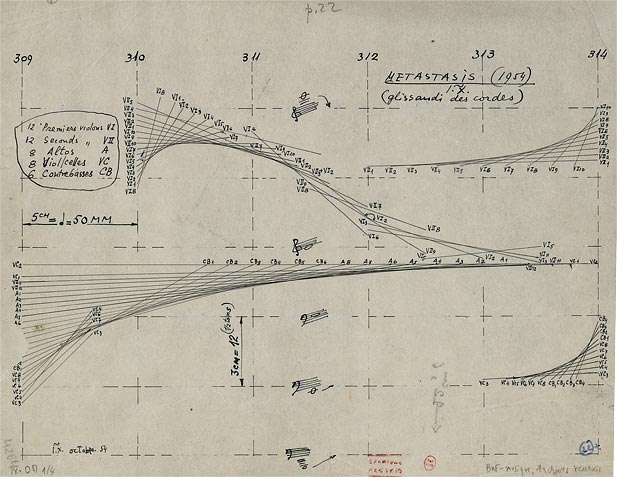
\includegraphics[width=\linewidth]{XenakisMetastasis.jpg}
  \caption{Excerpt from Iannis Xenakis' composition,
    \textit{Metastasis} (1954), measures 309-314. This score in this
    image was then transcribed to sheet music for the orchestral
    performance.}
  \label{fig:metastasis}
\end{figure*}

\subsection{The Philips Pavilion}
\label{sec:philips-pavilion-1}
\begin{figure}[h]
  \includegraphics[width=\linewidth]{PhilipsPavilion-TechnicalReview-01.pdf}
  \caption{The Philips Pavilion at the 1958 Brussels World Fair as
    shown in Volume 20 of the \textit{Philips Technical Review}, 1959}
  \label{fig:philips-pavilion-photo}
\end{figure}
In 1956, Le Corbusier was approached by Louis Kalff (Artistic Director
for the Philips corporation) and asked to build a pavilion for the
1958 World's Fair in Brussels. The pavilion was to showcase the sound
and lighting potential of Philips' technologies. Le Corbusier
immediately accepted, saying:
\begin{quotation}
  ``I will not make a pavilion for you but an Electronic Poem and a
  vessel containing the poem; light, color image, rhythm and sound
  joined together in an organic synthesis.''\cite{Lopez2011} 
\end{quotation}
The final product lived up to Le Corbusier's initial description. It
included:\cite{Lombardo2009}
\begin{enumerate}
\item A concrete pavilion, designed by architect and composer Iannis
  Xenakis
\item \textit{Interlude Sonoire} (later renamed \textit{Concret PH}), a
  tape music composition by Iannis Xenakis, approximately 2 minutes
  long, played between performances, while one audience left and
  pavillion, and the next audience another arrived.
\item A three channel, 8 minute tape music composition, by French-born
  composer Edgard Var\`{e}se
\item A system for spatialized audio across at least 350 loudspeakers
  distributed throughout the pavilion
\item An assortment of colored lighting effects, designed by Le Corbusier in
  collaboration with Philips art director Louis Kalff
\item Video consisting mostly of black and white still images,
  projected on two walls inside the pavilion
\item A system for synchronizing playback of audio and video,
  with the light effects and audio spatialization throughout the
  experience
\end{enumerate} 

\paragraph{The Role of Iannis Xenakis} During the initial design stage,
Le Corbusier determined that the shape of the pavilion building should
resemble a stomach, with the audience entering through one entrance,
and exiting through another. He completed initial sketches of the
pavilion layout, and then delegated the remainder of the design to
Xenakis.\cite{Clarke2012}

The architectural evolution of the pavilion from Le Corbusier's early
designs (figure~\ref{fig:le-corbusier-sketch}) through Xenakis'
iterations (figure~\ref{fig:xenakis-draw}), illustrates the impact
that Xenakis had on the project. An article in the \textit{Philips
  Technical Review}\cite{philips1958} gives a wonderfully detailed
account of Xenakis' process:
\begin{enumerate}
\item Xenakis was aware that parallel walls, or concave spherical
  walls would negatively impact audio perceptibility due to repeated
  or localized acoustic reflections.
\item To accommodate musical purpose of the space he decided to
  explore surfaces with varying curvature...
\item 
  \begin{marginfigure}
    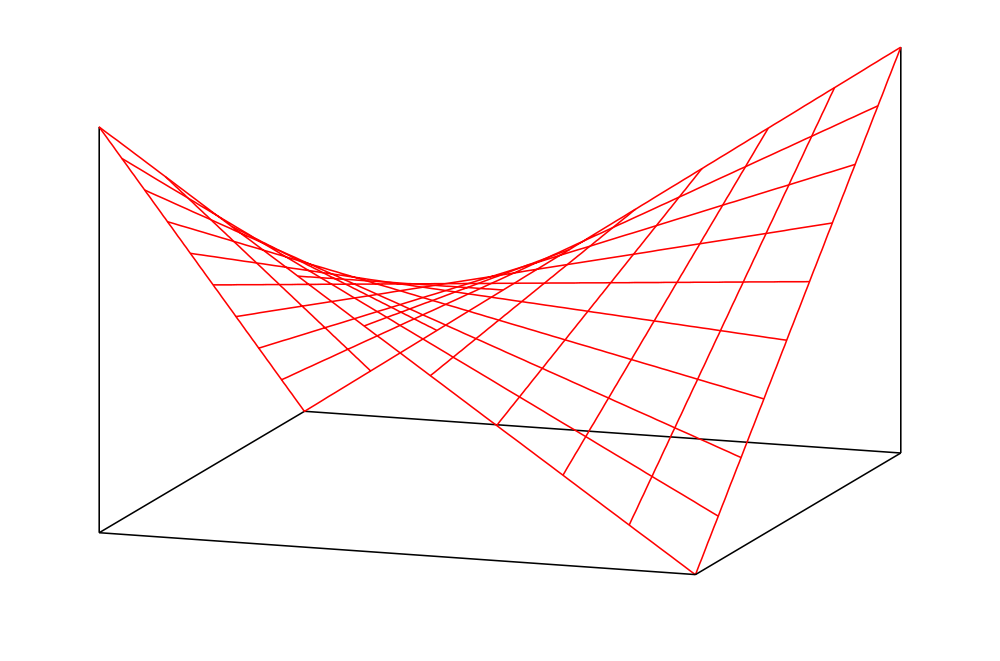
\includegraphics{hyperbolic-paraboloid}
    \caption{A ruled surface. For a surface to be considered ``ruled''
      every point on the surface must be on a straight line, and that
      line must lie on the surface. In Xenakis' time, ruled surfaces
      were useful in architecture, because they simplified the
      construction of curved surfaces by using straight beams.}
    \label{fig:ruled-surface}
  \end{marginfigure}...leading him to consider ruled surfaces such as
  the conoid and hyperbolic paraboloid. 
\end{enumerate}
We see Xenakis utilizing the drafting skills that he learned at the
Polytechnic Institute and continued to develop while working with Le
Corbusier. He also understood the mathematical formation of the ruled
surfaces that make up the structure. These surfaces even look familiar
from the Metastasis score (figure~\ref{fig:metastasis}). In his book
1963 book, \textit{Formalized Music}, Xenakis explicitly states that
the philips pavilion was inspired by his work on
\textit{Metastasis}.

\begin{figure*}[]
  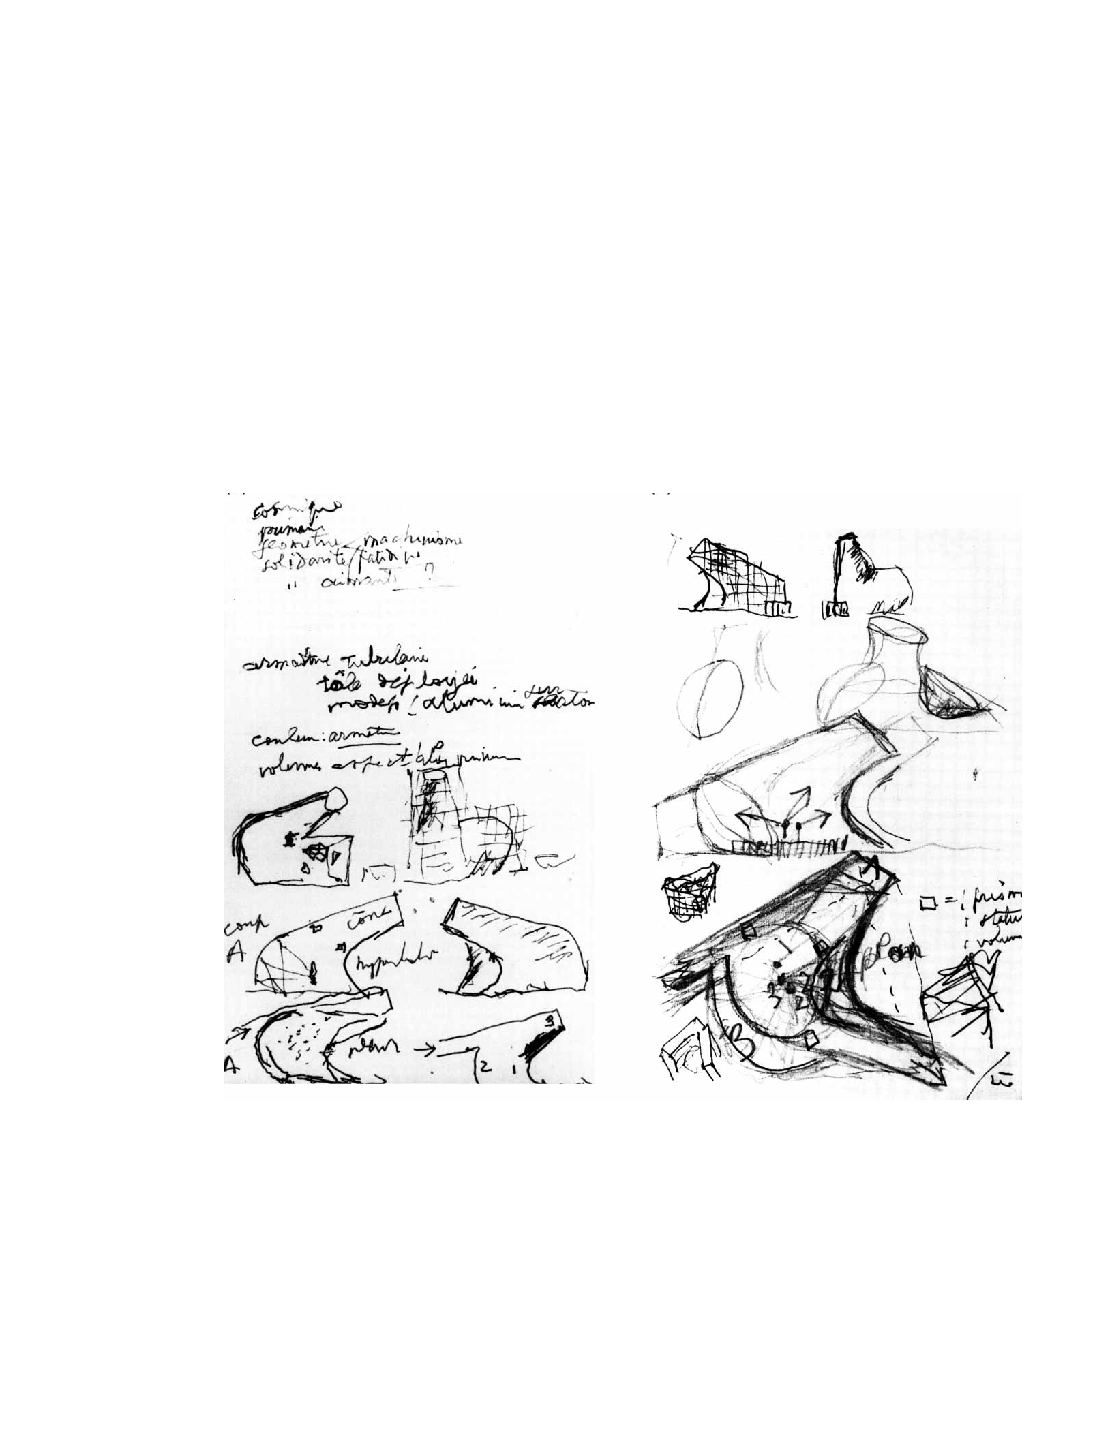
\includegraphics[width=\linewidth]{LeCorbusierDraw.pdf}
  \caption{Le Corbusier's design sketches for the Philips Pavilion,
    September \textendash{} October, 1956 (\textcircled{c} 2012
    Artists Rights Society, New York/ADAGP, Paris/FLC)}
  \label{fig:le-corbusier-sketch}
\end{figure*}

\begin{figure*}[h]
  % XenakisSketch.pdf or PhilipsDrawings.jpg
  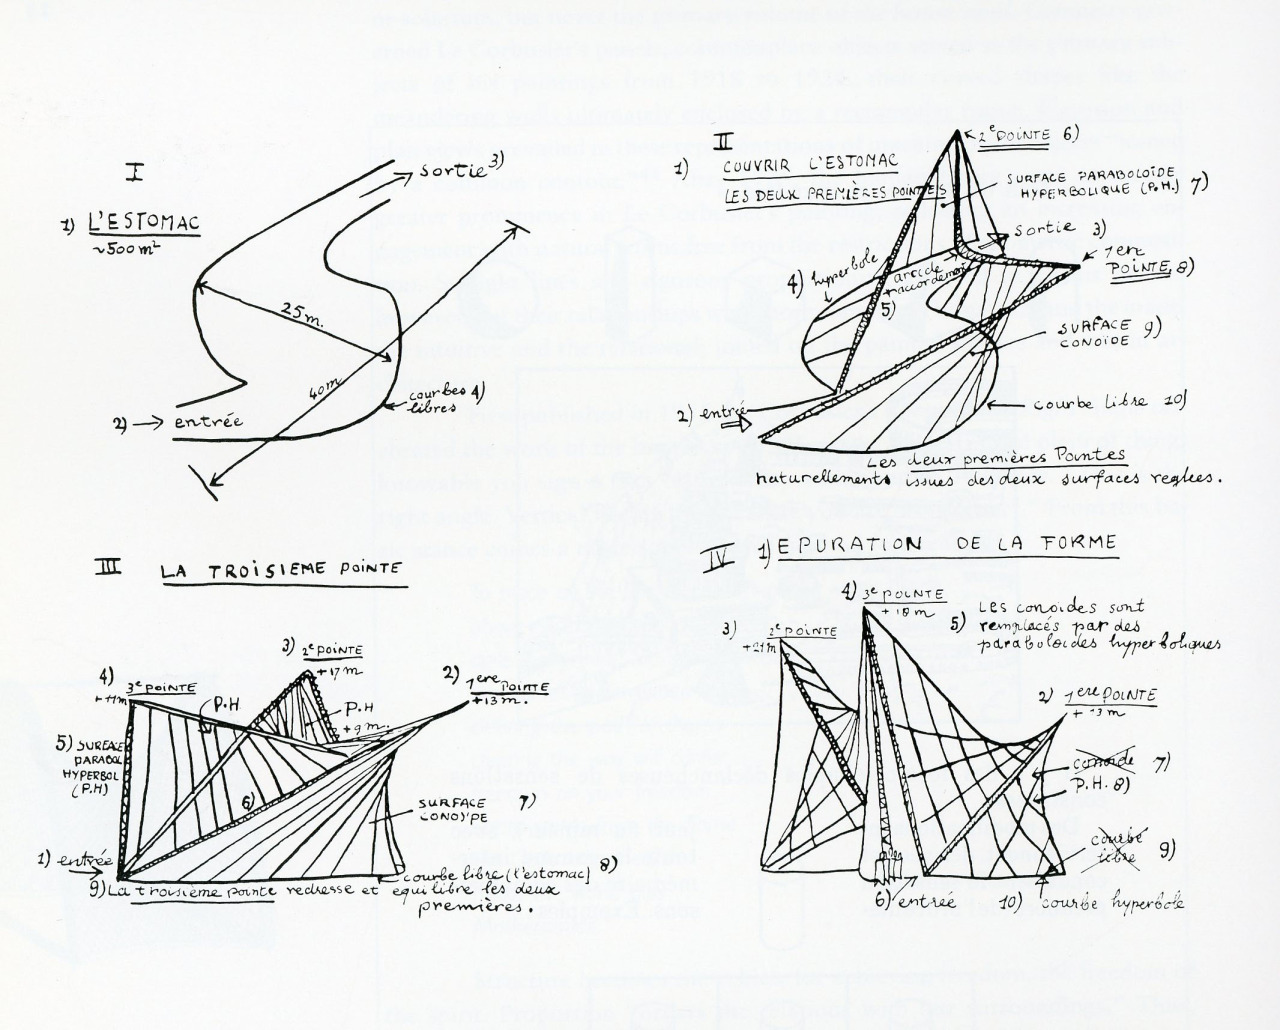
\includegraphics[]{PhilipsDrawings.jpg}
  \caption{Xenakis' early drawings of the Philips Pavilion as
    documented in volume 20 of the \textit{Philips Technical Review}.}
  \label{fig:xenakis-draw}
\end{figure*}

\section{Architecture and Music in Space and Time}
\label{sec:introduction-conclusion}

In \textit{Formalized Music},\cite{xenakis1992formalized} Xenakis
describes how developments in music theory mimic equivalent
developments in philosophy, mathematics, and the sciences. Plato, for
example, believed that all events transpire as determined by cause and
effect. While Plato and Aristotle both described causality in their
writing, it was not until the 17th century that controlled experiments
and mathematics corroborated the theory.\sidenote{In 1687, Isaac
  Newton published \textit{Philosophi\ae{} Naturalis Principia
    Mathematica} (\textit{Mathematical Principles of Natural
    Philosophy}), in which he compiled the 3 laws of motion that set
  the foundation for the study of \emph{classical mechanics}.}
Similarly, historical music follows deterministic progressions, and
music theory employs causal rules to describe counterpoint, tonality,
and harmonic movement.

Causality was largely used to describe physical phenomena until the
19th century when statistical theories in physics began to include
probabilistic notions.\sidenote{The Maxwell-Boltzmann distribution,
  which was first derived by James Clerk Maxwell in 1860, describes
  the probability distribution for the speed of a particle within an
  idealized gas. For more see
  \url{http://plato.stanford.edu/entries/statphys-statmech/}} Xenakis
noticed that more contemporary fields like \emph{probability theory}
and \emph{fuzzy logic} generalize and expand on the antecedent
theories of causality.

Xenakis thought that music composition should naturally follow
the progression that physics did, with the theory of music
generalizing and expanding on causal rules that had existed
previously. Indeed, starting in the late 19th century, and early 20th
century, composers like Strauss and Debussy began to bend the existing
rules of music theory, composing music that branched away from the
causal and tonal theories of the time. With the rise of
serialism\sidenote{Serialism is a technique for musical composition in
  which instances of musical elements (such as pitch, dynamics, or
  rhythm), are given numerical values. Sequences built from the values
  are ordered, repeated and manipulated throughout the composition.}
and indeterminate music\sidenote{In music, indeterminacy refers to the
  use of chance (such as rolling dice, or flipping coins) as part of
  the compositional process.}, composers such as Strauss, Debussy,
Stockhausen, Boulez, John Cage, Aaron Copland, and B\'{e}la Bart\'{o}k
began to use probability and chance in composition, the same way that
physicists were using probability to describe the material
world. However, to Xenakis' mathematical mind, serial music was no
less causal than the music it intended to supersede. He described
serial music as embodying ``virtually absolute
determinism.''\cite{xenakis1992formalized} Xenakis saw music theory as
a sub-set of mathematics and algebra. While musicians have a different
vocabulary, they also use mathematical principles to describe and
compose music. Because he understood mathematics as well as music, he
was able to identify how even in serialism and indeterminate music,
composers were only utilizing a small subset of algebraic theory. In
his own music, Xenakis wanted to generalize and expand the causal
framework that musicians and theorists had been using to compose and
understand music. This paralleled the developments in physics and
mathematics that helped him to form his opinions about music theory.
As a reference to \emph{chance} or \emph{stochos} Xenakis coined the
term \emph{stochastic music} to describe his development.

In \textit{Formalized Music}, Xenakis formally explains stochastic
music. It should be noted that some authors have interpreted his
description more explicitly. In \textit{Audible Design}, Trevor
Wishart, describes the stochastic process used to compose stochastic
music as:
\begin{quotation}
  ``A process in which the probabilities of proceeding from one state,
  or set of states. to another, is defined. The temporal evolution of
  the process is therefore governed by a kind of weighted
  randomness. which can be chosen to give anything from an entirely
  determined outcome, to an entirely unpredictable
  one.''\cite{Wishart1994}
\end{quotation}
It could be that the lack of a single clear definition by Xenakis is
the reason that few composers today identify as writing stochastic
music.

\paragraph{Xenakis' Reflection} In the Spring of 1976, Xenakis was
defending his doctoral thesis at the University of Paris. A
translation of his defense includes this statement:
\begin{quotation}
  ``The artist-conceptor will have to be knowledgeable and inventive
  in such varied domains as mathematics, logic, physics, chemistry,
  biology, genetics, paleontology (for the evolution of forms), the
  human sciences, and history; in short, a sort of
  \emph{universality}, but one based upon, guided by and oriented
  toward forms and architectures.'' \cite{russolo1986art}
\end{quotation}
From Xenakis' drawings we can deduce that he used the same tools,
skills, and philosophy to imagine and conceive both music and
space. His approach elevated both forms, and blurred the distinction
between the two. Maybe if we had kept using pen and paper to design
buildings and write music, the reality today would be closer to the
ideal that he imagined. Today, software for creating architecture or
composing music still favor corners to curves, and static pitches to
glissandi. More importantly, the software skills that we use to design
and manipulate space, and the skills that we use to compose music
mutually exclude each other.

This is where the projects described here make a contribution. As the
ideas that inspired Xenakis and other progressive 20th century
composers were taking root in contemporary music, the culture of
artistic form and composition was already beginning the transition
into the digital domain. However, there is no reason why digital tools
cannot favor stochastic procesees to linearity. There is no reason why
digital tools cannot treat music and architecture as equals. By
drawing from music, mathematics, computer science, acoustics, audio
engineering and mixing, sound reinforcement, multimedia production,
and live performance, we can create tools that allow us to
indiscriminately compose with space and sound.

\section{Universality}
\label{sec:universality}
At the MIT Media Lab, we celebrate the study and practice of projects
that exist outside of established academic disciplines. The Media Lab
(and the media) have described this approach as interdisciplinary,
cross-disciplinary, anti-disciplinary, or post-disciplinary;
emphasizing the clich\'{e} that traditional academics must become
experts in their field, and while narrowing their focus, they learn
\textit{more and more about less and less}, and eventually know
\textit{everything about nothing}.  \thesis is truly a Media Lab
project. It documents the creative process throughout the design,
development, and performance of a new type of audio signal
processor. In doing so, it draws from music, mathematics, computer
science, acoustics, audio engineering and mixing, sound reinforcement,
multimedia production, and live performance. How can we describe and
document a project with such broad subject material? Within a single
discipline, there is an accepted hierarchy of concepts, and we are
expected to develop a \emph{deep} understanding that penetrates this
hierarchy. We expect students to be literate in algebra, geometry and
calculus before studying physics. When we describe a physics problem,
we depend on an established collection of language, notation, and
theory.

This example reveals the curious tension between breadth and depth:
The \textit{depth} of a disciplinary approach provides the language
and abstraction that enable us to describe content and communicate at
a high level. Depth is essential for solving non-trivial
problems. However, solutions to the most complex and interesting
real-world projects always span multiple disciplines. It appears we
need breadth \emph{and} depth simultaneously.

One of the goals of this thesis is to bridge disciplines by describing
the material in a way that is accessible to readers that are not
experts in the all the fields involved. The work of Iannis Xenakis is
the perfect frame of reference because of it's powerful impact on
architecture, music, and culture.



\TODO{
The success of the Philips
Pavilion suggests the inherent value of the }


The challenge is to describe interdisciplinary projects so that it is
accessible to readers from all disciplines. This thesis proposes the
motivation for documenting media that exists outside of established
disciplines. It proposes a strategy for such documentation, and
employs this strategy by documenting the theory, implementation, and
application of \thesis.



%%% Local Variables:
%%% mode: latex
%%% TeX-master: "CharlesHolbrow_MAS_Thesis"
%%% End:

\clearpage
\chapter{Background}
\label{ch:background}
In this chapter, we review the precedent for contemporary explorations
of time and space in music. While far too many projects exist to cover
them all, we focus on projects that are either particularly impactful or
particularly relavant to the projects described in this thesis. We
conclude with a study of Iannis Xenakis' involvement in the
Philips Pavilion at the 1958 Brussels World Fair, which made
particularly innovative use of sound and space.

\paragraph{Early Spatial Music} Western spatial music emerged during
the renaissance period. The earliest published example of spatial
music was by Adrian Willaert in 1550.\cite{Zvonar1999} The Basilica
San Marco in Venice, where Willaert was \textit{maestro di capella},
had an interesting feature: two separate pipe organs facing each other
across the chapel. Willaert took advantage of this unusual setup by composing
music for separate choirs and instrumental groups adjacent the two
organs. Spatially separate choirs soon became a fashion and gradually
spread beyond Venice, as more and more spatially separated groups were
incorporated into composition. In honor of Queen Elizabeth's 40th
birthday in 1573, Thomas Tallis composed \textit{Spem in alium}, a
choral piece with 40 separate parts arranged in eight spatially
separated choirs. Interest in spatial composition declined
toward the end of the Baroque period, and was largely avoided until
the Romantic period. Beriloz' \textit{Requiem} in 1837, Giuseppe
Verdi's \textit{Requiem} in 1874, and Mahler's \textit{Symphony No. 2}
in 1895 all feature spatially separated brass ensembles.

\paragraph{Tempo Acceleration and Deceleration}
Chapter \ref{ch:polytempic} \marginnote{Do not to confuse polytempic
  music with poly\textit{metric} and poly\textit{rhythmic}
  music. Polyrhythms and polymeters are common in West
  African musical tradition and appear much earlier in Western music
  than polytempi.}  is concerned with oblique, similar, and contrary
tempo accelerations and decelerations in the context of polytempic
(with two or more simultaneous tempi) music.  The tempo indicators
commonly seen today, such as \textit{allegro} and \textit{adagio}, emerged
during the 17th century in Italy. While these markings partly express
a mood (\textit{gaily} and \textit{with leisure}, respectively), rather
than a strict tempo, they where much easier to follow than the
proportional system (based on tempic ratios such as 3:2 and 5:4) that
they replaced.\cite{Sachs1953} The intentional use of gradual tempo
changes likely evolved from the unconscious but musical tempo
fluctuations of a natural human performance. We can see examples of
the purposeful manipulation of tempo in the Baroque
period. Monteverdi's \textit{Madrigali guerrieri} from 1638 includes
adjacent pieces: \textit{Non havea Febo ancora}, and \textit{Lamento
  della ninfa}. The score instructs to perform the former piece
\textit{al tempo della mano} (in the tactus of the conducting hand),
and the latter \textit{a tempo del'affetto del animo e non a quello
  della mano} (in a tempo [dictated by] emotion, not the hand).
While Monteverdi's use of controlled tempo was certainly not the
first, we are particularly interested in gradual tempo changes in
polytempic compositions, which do not appear in Western music until
near the beginning of the 20th century.

%\section{Wagner's Gessamtkunstwerk}

\section{20th Century Modernism}
\label{sec:modernism}
As the Romantic period was coming to an end, there was a blossoming of
complexity, diversity, and invention in contemporary music. While Performers
developed the virtuosic skills required to play the music, composers
also wrote increasingly difficult scores to challenge the
performers.\cite{Grout2006} Works by Italian composer Luciano Berio
illustrate the complexity of contemporary music of the time. Beginning
in 1958, Berio wrote a series of works he called
\textit{Sequenza}. Each was a highly of highly technical composition
written for a virtuosic soloist. Each was for a different instrument
ranging from flute to guitar to accordion.  In Sequenza~IV, for piano,
Berio juxtaposes thirty-second note quintuplets, sextuplets, and
septuplets (each with a different dynamic), over just a few
measures. 

\section{Polytempic Music}
\label{sec:background-polytempi}
Western polytempi can be traced to Henry Cowell's book, \textit{New Musical
  Resources}, first published in 1930, wherein Cowell states:
\begin{quotation}
  ``Rhythm presents many interesting problems, few of which have been
  clearly formulated. Here, however, only one general idea will be
  dealt with-namely, that of the relationship of rhythm, which have an
  exact relationship to sound-vibration, and, through this
  relationship and the application of overtone ratios, the building of
  ordered systems of harmony and counterpoint in rhythm, which have an
  exact relationship to tonal harmony and
  counterpoint.''\sidenote{Examples from \textit{New Musical
      Resources} are from the 3rd edition, published in
    1996.}\cite{Cowell1996}
\end{quotation}
Cowell goes on to describe a system of ratios for tempi: If we think
of two parallel tempi, one going twice the rate of the other, it is
akin to the octave pitch interval, one fundamental frequency being
twice the other. Similarly, the vibration ratio of 2:3 can be thought
of as a fifth, and some rhythmic relationships are ``harmonious'',
while others are ``dissonent.'' This is nearly identical to the
proportional tempo technique that was displaced in Italy in the 1600s,
but Cowell does eventually introduce the concept of polytempic music:
\begin{quotation}
``The use of different simultaneous tempi in a duet or quartet in opera,
for instance would enable each of the characters  to express his
individual mood; such a system might  effectively be applied to the
famous quartet from \textit{Rigoletto}, in which each of the
characters is expressing a different emotion.''
\end{quotation}
This example is closer to what we are interested in, but does not
include simultaneous tempo changes. However, Cowell takes the
idea a step further, illustrating the possibility of parallel tempo
acceleration with figure~\ref{fig:cowell-polytemp}.
\begin{marginfigure}
  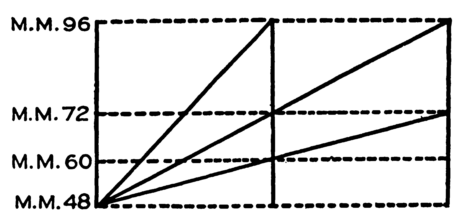
\includegraphics[width=\linewidth]{CowellPolytemp.png}
  \caption{Polytempic tempo transitions as illustrated by Henry Cowell
    in 1930. \textcircled{c} Cambridge University Press}
  \label{fig:cowell-polytemp}
\end{marginfigure}
While he was not a mathematician, Cowell did understand that there
were some unanswered complications surrounding simultaneous tempo
changes. While describing polytempic accelerations he notes:
\begin{quotation}
``For practical purposes, care would have to be exercised in the use of
sliding tempo, in order to control relation between tones in a sliding
part with those in another part being played at the same time: a
composer would have to know, in other words, what tones in a part with
rising tempo would be struck simultaneously with other tones in a part
of, say, fixed tempo, and this from considerations of harmony. There
would usually be no absolute coincidence, but the tones which would be
struck at approximately the same time could be calculated.''
\end{quotation}
It is possible to calculate exactly when tones in an accelerating
tempo will be struck. n the examples shown in
figure~\ref{fig:cowell-polytemp}, the linear tempo accelerations only
rarely yield satisfactory results. Figure~\ref{fig:cowell-polytemp}
does not show how many beats or measures elapse during the tempo
acceleration, but with linear acceleration shown, the parallel tempi
are likely to be out of phase once the tempo transition is
complete. This is described in more detail in \autoref{ch:polytempic}.

\subsection{Modernism and Rhythmic Complexity}
\label{sec:modern-rhythm-compl}
During the Modernist period, many composers sought new ways to use
time and space as compositional elements, and polytempic music was
relatively unexplored. Traditional music notation is not well-equipped
to handle acceleration with precision. The conventional way to
describe gradual tempichanges is to annotate the score with notes like
\textit{ritardando} (gradually slowing) and \textit{accelerando}
(gradually accelerating), coupled with traditional Italian tempo
markings like \textit{adagio} (slow, stately, at ease) and
\textit{allegro} (fast, quickly, bright). Exact tempo rates can be
explicitly specified with an M.M.\sidenote{In a musical score,
  M.M. stands for Maelzel's Metronome, and is accompanied by a number
  specifying the beats per minute.}  marking. It is not realistic to
expect a performer to be able to follow a precise mathematical
acceleration. This did not stop modernist composers from finding
creative ways to notate surprisingly precise polytempic compositions
using only the conventional notation:
\begin{enumerate}
\item Groups of tuplets layered against a global tempo, as used by
  Henry Cowell (\textit{Quartet Romantic}, 1915-17) and Brian Fernyhough
  (\textit{Epicycle for Twenty Solo Strings}, 1968).
\item Polymeters are notated against a global tempo, and the value of
  a quarter note is the same in both sections, as in Elliott Carter's \textit{Double
    Concerto for Harpsichord and Piano with Two Chamber Orchestras}, 1961
  and George Crumb's \textit{Black Angels}, 1971.
\item Sections are notated without meter. Notes are positioned
  horizontally on the leger linearly, according to their position in
  time. Conlon Nancarrow (\textit{Study No. 8 for Player Piano},
  1962) and Luciano Berio (\textit{Tempi Conceriati}, 1958-59).
\item The orchestra is divided into groups, and groups are given
  musical passages with varying tempi. The conductor cues groups to
  begin (Pierre Boulez, \textit{Rituel: In Memoriam Maderna},1974).
\item One master conductor directs the entrances of auxiliary
  conductors, who each have their own tempo and direct orchestral
  sections (Brant Henry, \textit{Antiphony
    One for Symphony Orchestra Divided into 5 Separated Groups}, 1953).
\end{enumerate}

\subsection{Charles Ives and The Unanswered Question}
\label{sec:charles-ives}
One composer, Charles Ives, did write polytempic music before \textit{New Musical
  Resources} was published. Ives was an American composer
whose works were largely overlooked during his lifetime. One of these,
his 1908 composition, \textit{The Unanswered Question}, is remarkable in
that it incorporates both spatial and polytempic elements. In this
piece, the string section is positioned away from the stage, while the
trumpet soloist and woodwind ensemble are on the stage. A dialogue
between the trumpet, flutes, and strings is written into the music,
with the trumpet repeatedly posing a melodic question \textit{"The
  Perennial Question of Existence.''} Each question is answered by the
flute section. The first response is synchronized with the trumpet
part, but subsequent responses accelerate and intentionally
desynchronize from the soloist. Ives included a note at the beginning
of the score which describes the behavior of the ``The Answers'':
\begin{quotation}
This part need not be played in the exact time position indicated. It
is played in somewhat of an impromptu way; if there is no conductor,
one of the flute players may direct their playing.

The flutes will end their part approximately near the position
indicated in the string score; but in any case, "The Last Question"
should not be played by the trumpet until "The Silences" of the
strings in the distance have been heard for a measure or two. The
strings will continue their last chord for two measures or so after
the trumpet stops. If the strings shall have reached their last chord
before the trumpet plays "The Last Question", they will hold it
through and continue after, as suggested above.

"The Answers" may be played somewhat sooner after each "Question" than
indicated in the score, but "The Question" should be played no sooner
for that reason.
\end{quotation}
Ives gave the performers license over the temporal alignment, but he
made it clear that the parts should not be played together. 

% Following Ives, other modernist composers also sought new ways to
% manipulate tempo and meter.

\subsection{Gruppen}
\label{sec:gruppen}
Ives' polytempic compositions from the first half of the 20th century
are somewhat of an exception. Polytempi was not widely explored until
well after \textit{New Musical Resources} was published. One famous
example is Karlheinz Stockhausen's \textit{Gruppen} for three
orchestras (1955-57). Managing parallel tempi that come in and out of
synchronicity is always a challenge with polytempic music, and
Stockhausen found an effective, if heavy-handed, solution with a
system of discrete tempo changes. Each of the three orchestras was to
have it's own conductor, and the conductor would listen for a cue
carefully written in one of the other sections. That cue would signal
to the conductor to begin beating a silent measure at the new tempo
and prepare the new orchestra to begin playing.  Stockhausen did not
say that he was inspired by \textit{New Musical Resources} directly,
but his famous essay \textit{How Time Passes} describes how he chose
the tempic ratios used in \textit{Gruppen}. Instead of basing the
tempo scales on simple pythagorean relationships, Stockhausen chose
the relationships based on the $\sqrt[12]{2}$ ratio of adjacent notes
in equal tempered tuning.


\subsection{Conlon Nancarrow}
\label{sec:conlon-nancarrow}
Conlon Nancarrow is best known for his incredibly complex player piano
scores, and is recognized as one of the first composers to realize the
potential of technology to perform music beyond human capacity. Unlike
Stockhausen, Nancarrow did acknowledge the influence of Cowell's
\textit{New Musical Resources} on his own works. His compositions for
the player piano, beginning with \textit{Study for Player Piano
  No. 21}, did incorporate polytempic
accelerations\cite{Rao2005}. While some of Nancarrow's compositions do
feature many simultaneous tempi, (Study No. 37 features 12
simultaneous tempi)\cite{Greschak2003}, a rigorous mathematical
approach would be required for all 12 tempi to accelerate or
decelerate relative to each other and synchronize at pre-determined
points. Interestingly, Nancarrow said in a 1977 interview that he was
originally interested in electronic music, but the player piano gave
him more temporal control.\cite{Amirkhanian1977}

% William Duckworth
% The Time Curve Preludes
% https://en.wikipedia.org/wiki/William_Duckworth_(composer)

\subsection{New Polytempi}
\label{sec:new-polytempi}
The many different approaches to polytempi in modernist music all
have one thing in common: They all wrestle with synchronicity. Human
performers are not naturally equipped to play simultaneous tempi, and
composers must find workarounds that make polytempic performance
accessible.

The examples described in this chapter exist in one or more of the
following categories:
\begin{enumerate}
\item The tempo changes are discrete rather than continuous.
\item The music may suggest multiple tempi, bar lines of parallel 
  measures line up with each other, and the ``changing'' tempi are 
  within a global tempo. 
\item The tempo changes are somewhat flexible, and  the exact number of
  beats that elapse during a transition varies from one performance to
  another.
\item The tempo acceleration is linear, and parallel parts align only at simple
  mathematical relationships.
\end{enumerate}
It is not simple to rigorously define parallel tempo curves that
accelerate and decelerate continuously relative to each other, and
come into synchronicity at strict predetermined musical points for all
voices. In \autoref{ch:polytempic}, we discuss how existing electronic
and acoustic music approaches this challenge, and derive a
mathematical solution that unlocks a previously inaccessible genre of
polytempic music.

\section{Amplified Spatial Music}
\label{sec:spatial-developments}
The evolution of polytempic music in the Modernist period was
paralleled by innovation in the creation and performance of electronic
music. After World War II, new technology became available to
composers, and with this new technology came new styles of music.
Pierre Schaeffer was among the first composers using electronic sounds
together with acoustic ones.  He worked at the
Radiodiffusion-T\'{e}l\'{e}vision Fran\c{c}aise (RTF), where he helped
to pioneer early practices in musique concr\`{e}te. With the help of
younger composer Pierre Henry, he was also among the first composing
spatialized pre-recorded sound. The pair collaborated on a piece
called \textit{Symphonie pour un Homme Seul} (Symphony for One Man
Alone, 1950). For this piece they created a tetrahedral loudspeaker
arrangement and a rather dramatic interface that they called the
\textit{Pupitre d'espace}, shown in figure~\ref{fig:schaeffer}. Large
hoops on the device had inductive coils that sensed the user's hand
position and controlled the signal routing to the
loudspeakers.\cite{Holm2008}
\begin{marginfigure}
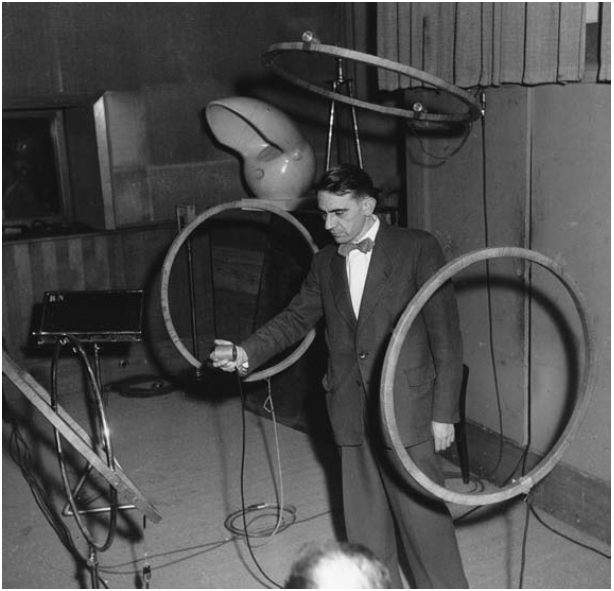
\includegraphics{Schaeffer.png}
\caption{Pierre Schaeffer with the \textit{Pupitre d'espace} in
  1951. \textcircled{c} Ina/Maurice Lecardent, Ina GRM Archives}
\label{fig:schaeffer}
\end{marginfigure}


\subsection{Gesang der J\"{u}nglinge}
The success of Schaeffer's music at the RTF attracted the attention of
other composers interested in electronic music. Among them was
Karlheinz Stockhausen. Stockhausen came to RTF and composed just one
2-track etude in 1952 before returning to West Germany, where he
continued to compose orchestral and electronic works. His practice led
to the composition of what is widely regarded as the first masterpiece
of electronic music, \textit{Gesang der J\"{u}nglinge} (Song of the
Youths, 1955-56), which was also the first multichannel pre-recorded
composition to be performed in a concert setting with multiple
loudspeakers placed around the audience\cite{Grout2006}. 

The piece stands out by the many aspects in which it is both
evolutionary and revolutionary when juxtaposed with the other
electronic compositions of the time; the delicate blending of the
voice with electronics, and the creative editing of the voice being
two examples. It has been extensively analyzed and reviewed in
literature;\cite{Decroupet1998,Metzer2004,Miller2009} however, the
exact strategy for the spatialization of sound in the original
four-channel performance remains somewhat ambiguous. From interviews
and essays with Stockhausen, we can gather some insight into his
process. In 1955, the year when Stockhausen began work on
\textit{Gesang der J\"{u}nglinge}, he published an essay on his serial
technique.
\begin{quotation}
``By regulating the positions of the sources of sound it will be
possible for the first time to appreciate aesthetically the universal
realisation of our integral serial technique.''\cite{Stockhausen1955}
\end{quotation}
In an interview published in 1974 he made the following comment on the
subject of sound positioning in \textit{Gesang der J\"{u}nglinge}:
\begin{quotation}
  ``The speed of the sound, by which one sound jumps from one speaker to
  another, now became as important as pitch once was. And I began to
  think in intervals of space, just as I think in intervals of pitch
  or durations. I think in chords of space.''\cite{Stockhausen1974}
\end{quotation}
A side effect of serialism is discouraging the uneven distribution of
a musical parameter. With this in mind, spatialization is a very
natural target for serialism. Given the added creative flexibility of
surround sound, it reasonable to search for ways to take full
advantage of the new dimension, without favoring any particular
direction or loudspeaker.

\begin{figure}
  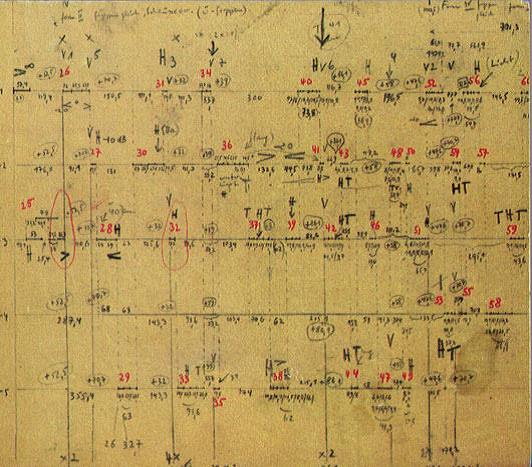
\includegraphics{Gesang.jpg}
  \caption{Excerpt from the \textit{Gesang der J\"{u}nglinge}
    manuscript. \textcircled{c}~www.karlheinzstockhausen.org}
  \label{fig:schaeffer-score}
\end{figure}

\subsection{Advances in Surround Panning}
\label{sec:advanc-surr-pann}
For his next four-track tape composition, \textit{Kontakte}
(1958-60), Stockhausen devised a new technology that made it quite
simple to continuously pan sounds between the speakers orbiting the
listener. He used a rotating speaker on a turntable, surrounded by
four equally spaced microphones. Stockhausen continued to feature
spatialization prominently in both acoustic and electronic work.  His
major orchestral compositions, \textit{Gruppen} (1955-57, described in
section~\ref{sec:gruppen}) and \textit{Carr\'{e}} (for four orchestra
and four choirs, 1959-60) both prominently feature spatialization.

Throughout the rest of the century, advances in technology enabled new
performances with more speakers and more complex spatial
possibilities. The Vortex multimedia program at the Morrison
Planetarium in San Francisco (1957-59) featured 40 loudspeakers with
surround sound panning, facilitated by a custom rotary console, and
featured works by Stockhausen, Vladimir Ussachevsky, Toru Takemitsu,
and Luciano Berio. The planetarium featured synchronized lighting,
which became a hallmark of major surround sound productions of the
time. The Philips Pavilion at the 1958 Brussels Worlds' Fair used a
custom sequencer hooked up to a telephone switcher to pan sounds
between over 300 speakers (more in
section~\ref{sec:philips-pavilion-1}).  John Chowning's
\textit{Turenas}, (1972) simulated amplitude changes and doppler shift
of sound objects' movements as a compositional
element.\cite{Chowning2011} The West German pavilion at Expo 70 in
Osaka, Japan, included a dome 28 meters in diameter, five hours of
music composed by Stockhausen, and 20 soloist musicians. Stockhausen
``performed'' the live three-dimensional spatialization from a custom
console near the center of the dome (figure~\ref{fig:stockhausen-expo}).
\begin{figure}
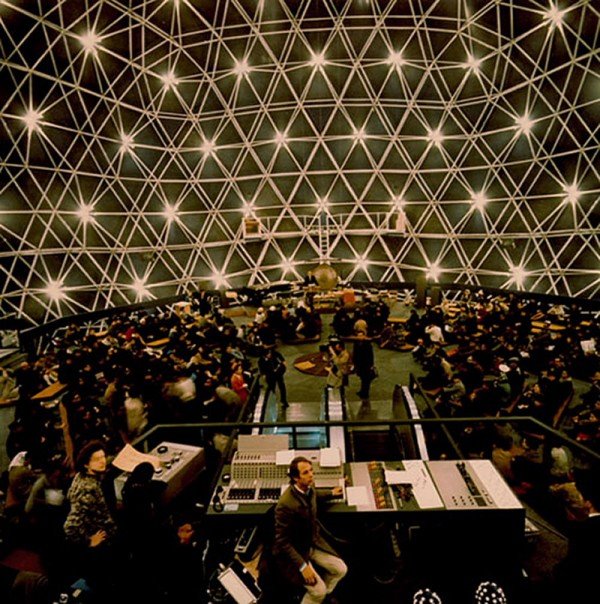
\includegraphics{Expo70.jpg}
\caption{Inside the West Greman pavillion at Expo 70. Osaka, 1970.}
\label{fig:stockhausen-expo}
\end{figure}
The West German dome was not the only massive spatialized sound
installation at Expo 70. Iannis Xenakis, the mastermind behind the
1958 Philips Pavilion in Brussels, was also presenting his 12-channel
tape composition, \textit{Hibiki Hana Ma}, at the Japanese Steel
Pavilion through 800 speakers positioned around the audience,
overhead, and underneath the seats. 

%\TODO{Ambisonics, Commercial options like Dolby}

\subsection{Evolution of Electronic Composition}
\label{sec:evolution-of-electronic-composition}
\textit{Gesang der J\"{u}nglinge} may have been the first masterpiece
of electronic music, but the techniques that were developed at the RTF
studios were quickly spreading. Another composer who was drawn to RTF
(where musique concr\`{e}te was first conceived by Pierre Schaeffer)
was Pierre Boulez. However, Boulez was generally unsatisfied with his
early electronic compositions and frustrated by the equipment required
to make electronic music. Despite his general distaste for electronic
music composition, Boulez was approached by the French President,
Georges Pompidou, in 1970 and asked to found an institution dedicated
to the research of modern musical practice. The center, IRCAM, opened in 1977
with Boulez at the head. In a 1993 interview, Boulez described how he
directed the efforts of the lab:
\begin{quotation}
  ``Back in the 1950s, when you were recording sounds on tape and using
  them in a concert, you were merely following the tape, which became
  very detrimental to the performance. So I pushed the research at
  IRCAM to examine the use of live electronics, where the computer is
  created for the concert situation, instantly responding to your
  actions. The system's language also became easier to follow; I
  remember when I tried to learn the electronics, it was all figures,
  figures, figures. These meant nothing at all to the musician. If you
  have to work in hertz and not notes, and then wait half an hour to
  process the sounds, you get completely discouraged. My goal was so
  that the musician could sketch his ideas very rapidly, with
  instantaneous sound and graphical notation. The use of computers
  finally brought electronics down to the level of understanding for
  composers. I feel very responsible for that change.''\cite{Carvin1993}
\end{quotation}
Boulez' first major composition that took advantage of the resources
at IRCAM was \textit{R\'{e}pons} which premiered at the Donaueschingen
Festival in Germany in 1981 (allthough Boulez continued to revise it
until 1984). The piece balances 24 acoustic performers with
pre-recorded material and live processing with spatialization over a
ring of 38 loudspeakers. The audience sits in a circle surrounding the
orchestra, while six of the acoustic instrumentalists are spaced
around the outside of the audience. Boulez was certainly not the first
composer to mix elextronics with acoustic performers (Milton
Babbitt's 1964 \textit{Philomel} is a much earler example), but
\textit{R\'{e}pons} does mark a certain maturity of the form.

% Janet Cardif? 40 part motet wasn't until 2001
% \TODO{Berio, Boulez (repons), Stockhausen (Gesang der Junglinge), etc}

\section{Iannis Xenakis}
\label{sec:iannis-xenakis}
The projects in this thesis build on the work and ideas of Iannis
Xenakis. Xenakis studied music and engineering at the Polytechnic
Institute in Athens, Greece. By 1948, he had graduated from the
university and moved to France where he began working for the French
architect, Le Corbusier. The job put his engineering skills to use,
but Xenakis also wanted to continue studying and writing music. While
searching for a music mentor, he approached Oliver Messiaen and asked
for advice on whether he should study harmony or
counterpoint. Messiaen was a prolific French composer known for
rhythmic complexity. He was also regarded as a fantastic music
teacher, and his students included Stockhausen and Boulez. Messiaen
later described his conversation with Xenakis:
\begin{quotation}``I think one should study harmony and
  counterpoint. But this was a man so much out of the ordinary that I
  said: No, you are almost 30, you have the good fortune of being
  Greek, of being an architect and having studied special
  mathematics. Take advantage of these things. Do them in your
  music.''\cite{Service2013}
\end{quotation}
In essence, Messiaen was rejecting Xenakis as a student, but we can
see how Xenakis ultimately drew from his disparate skills in his
compositions. The score for his 1945 composition \textit{Metastasis}
(figure~\ref{fig:metastasis}) resembles an architectural blueprint as
much as it does a musical score.

\begin{figure*}[h]
  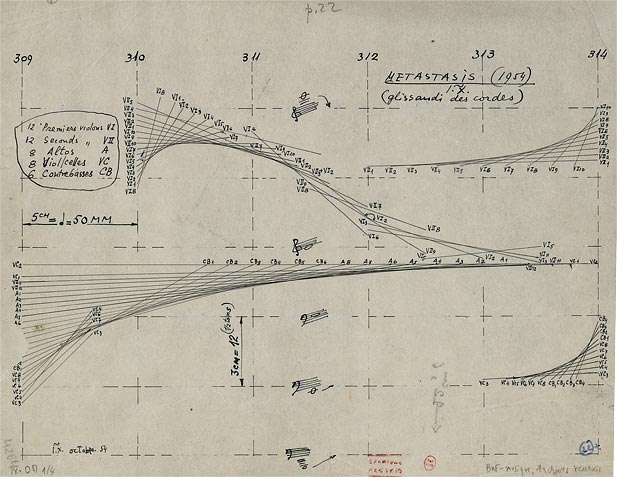
\includegraphics[width=\linewidth]{XenakisMetastasis.jpg}
  \caption{Excerpt from Iannis Xenakis' composition,
    \textit{Metastasis} (1954), measures 309-314. This score in this
    image was then transcribed to sheet music for the orchestral
    performance.}
  \label{fig:metastasis}
\end{figure*}

\subsection{The Philips Pavilion}
\label{sec:philips-pavilion-1}
\begin{figure}[h]
  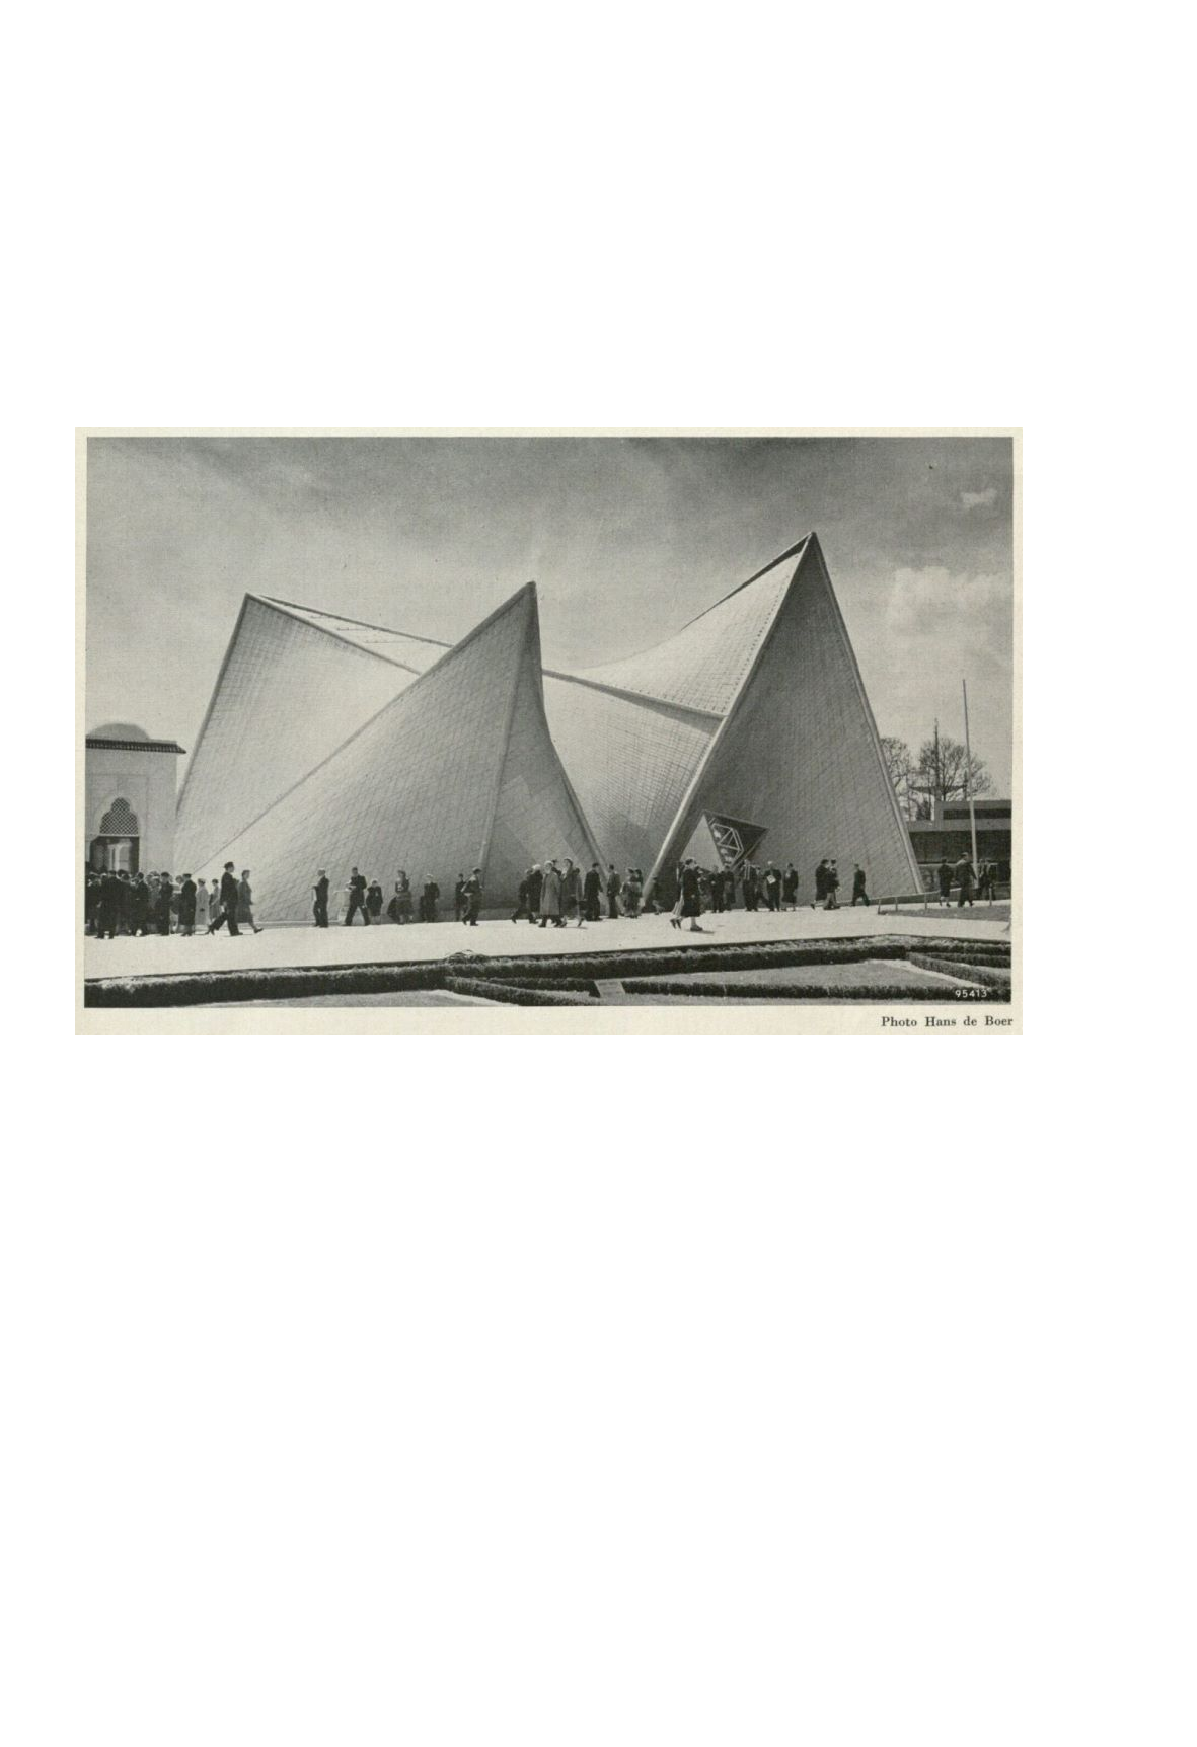
\includegraphics[width=\linewidth]{PhilipsPavilion-TechnicalReview-00.pdf}
  \caption{The Philips Pavilion at the 1958 Brussels World Fair as
    shown in Volume 20 of the \textit{Philips Technical Review}, 1959.}
  \label{fig:philips-pavilion-photo}
\end{figure}
In 1956, Le Corbusier was approached by Louis Kalff (Artistic Director
for the Philips corporation) and asked to build a pavilion for the
1958 World's Fair in Brussels. The pavilion was to showcase the sound
and lighting potential of Philips' technologies. Le Corbusier
immediately accepted, saying:
\begin{quotation}
  ``I will not make a pavilion for you but an Electronic Poem and a
  vessel containing the poem; light, color image, rhythm and sound
  joined together in an organic synthesis.''\cite{Lopez2011} 
\end{quotation}
The final product lived up to Le Corbusier's initial description. It
included:\cite{Lombardo2009}
\begin{enumerate}
\item A concrete pavilion, designed by architect and composer Iannis
  Xenakis
\item \textit{Interlude Sonoire} (later renamed \textit{Concret PH}), a
  tape music composition by Iannis Xenakis, approximately 2 minutes
  long, played between performances, while one audience left the
  pavilion and the next audience arrived
\item \textit{Po\`{e}me \'{E}lectronique}, a three-channel, 8 minute
  tape music composition by composer Edgard Var\`{e}se
\item A system for spatialized audio across more than 350 loudspeakers
  distributed throughout the pavilion
\item An assortment of colored lighting effects, designed by Le Corbusier in
  collaboration with Philips' art director, Louis Kalff
\item Video consisting mostly of black and white still images,
  projected on two walls inside the pavilion
\item A system for synchronizing playback of audio and video,
  with light effects and audio spatialization throughout the
  experience
\end{enumerate} 

\paragraph{Role of Iannis Xenakis} During the initial design stage, Le
Corbusier decided that the shape of the pavilion should resemble a
stomach, with the audience entering through one entrance and exiting
out another. He completed initial sketches of the pavilion layout and
then delegated the remainder of the design to
Xenakis.\cite{Clarke2012}

The architectural evolution of the pavilion from Le Corbusier's early
designs (figure~\ref{fig:le-corbusier-sketch}) to Xenakis' iterations
(figure~\ref{fig:xenakis-draw}), illustrates the profound impact that
Xenakis had on the project. Xenakis was aware that parallel walls and
concave spherical walls could both negatively impact audio
perceptibility due to repeated or localized acoustic reflections. The
walls of the pavilion had to accomodate lighting effetcs, which were
projected from many different angles, leading him to consider sufaces
with a varying rate of curvature.\cite{philips1958}
  \begin{marginfigure}
    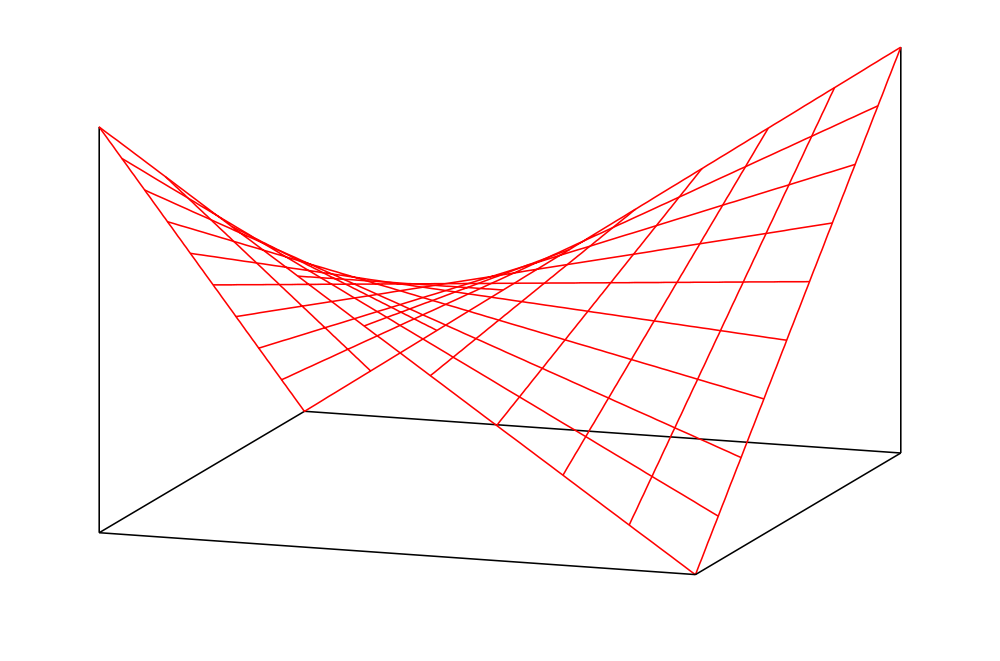
\includegraphics{hyperbolic-paraboloid}
    \caption{A ruled surface. For a surface to be considered ``ruled''
      every point on the surface must be on a straight line, and that
      line must lie on the surface. In Xenakis' time, ruled surfaces
      were useful in architecture, because they simplified the
      construction of curved surfaces by using straight beams.}
    \label{fig:ruled-surface}
  \end{marginfigure}
Ruled surfaces such as the conoid and hyperbolic paraboloid, seemed to
meet the needs of the project, and also acomodate the acoustical needs.
Through this process, we see Xenakis utilizing the skills that he
learned at the Polytechnic Institute and continued to develop while
working with Le Corbusier. He also understood the mathematical
formation of the ruled surfaces that make up the structure. These
surfaces even look familiar to the Metastasis score
(figure~\ref{fig:metastasis}). In his 1963 book, \textit{Formalized
  Music}, Xenakis explicitly states that the Philips Pavilion was
inspired by his work on \textit{Metastasis}.

\begin{figure*}[]
  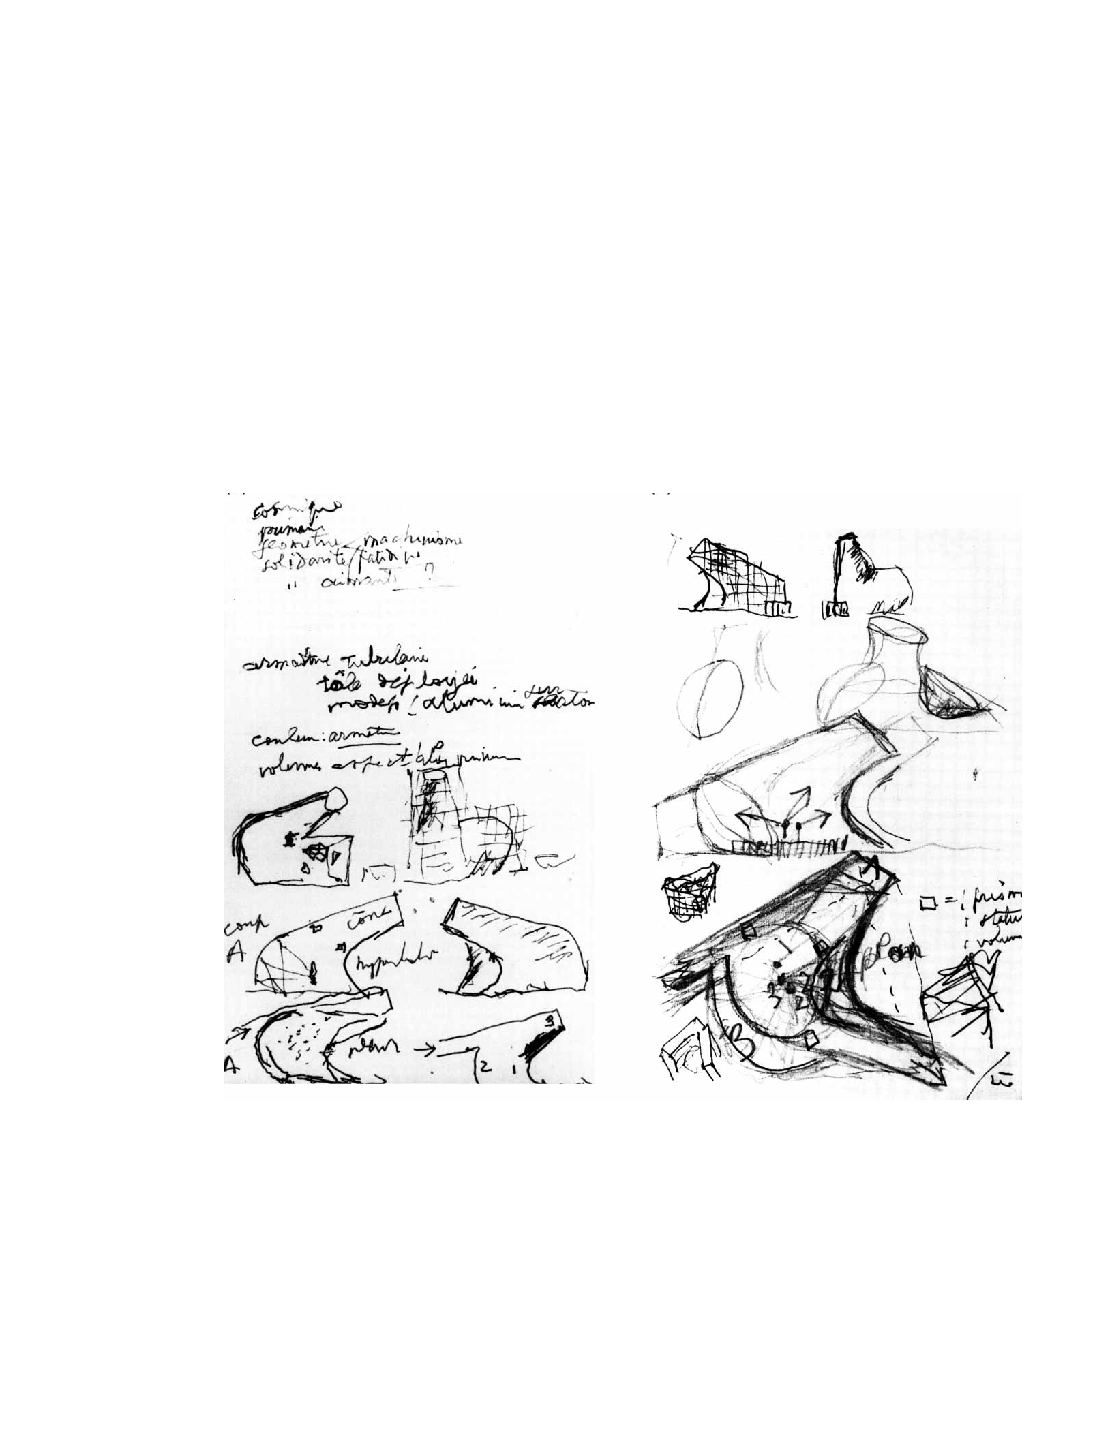
\includegraphics[width=\linewidth]{LeCorbusierDraw.pdf}
  \caption{Le Corbusier's design sketches for the Philips Pavilion,
    September \textendash{} October, 1956 (\textcircled{c} 2012
    Artists Rights Society, New York/ADAGP, Paris/FLC)}
  \label{fig:le-corbusier-sketch}
\end{figure*}

\begin{figure*}[h]
  % XenakisSketch.pdf or PhilipsDrawings.jpg
  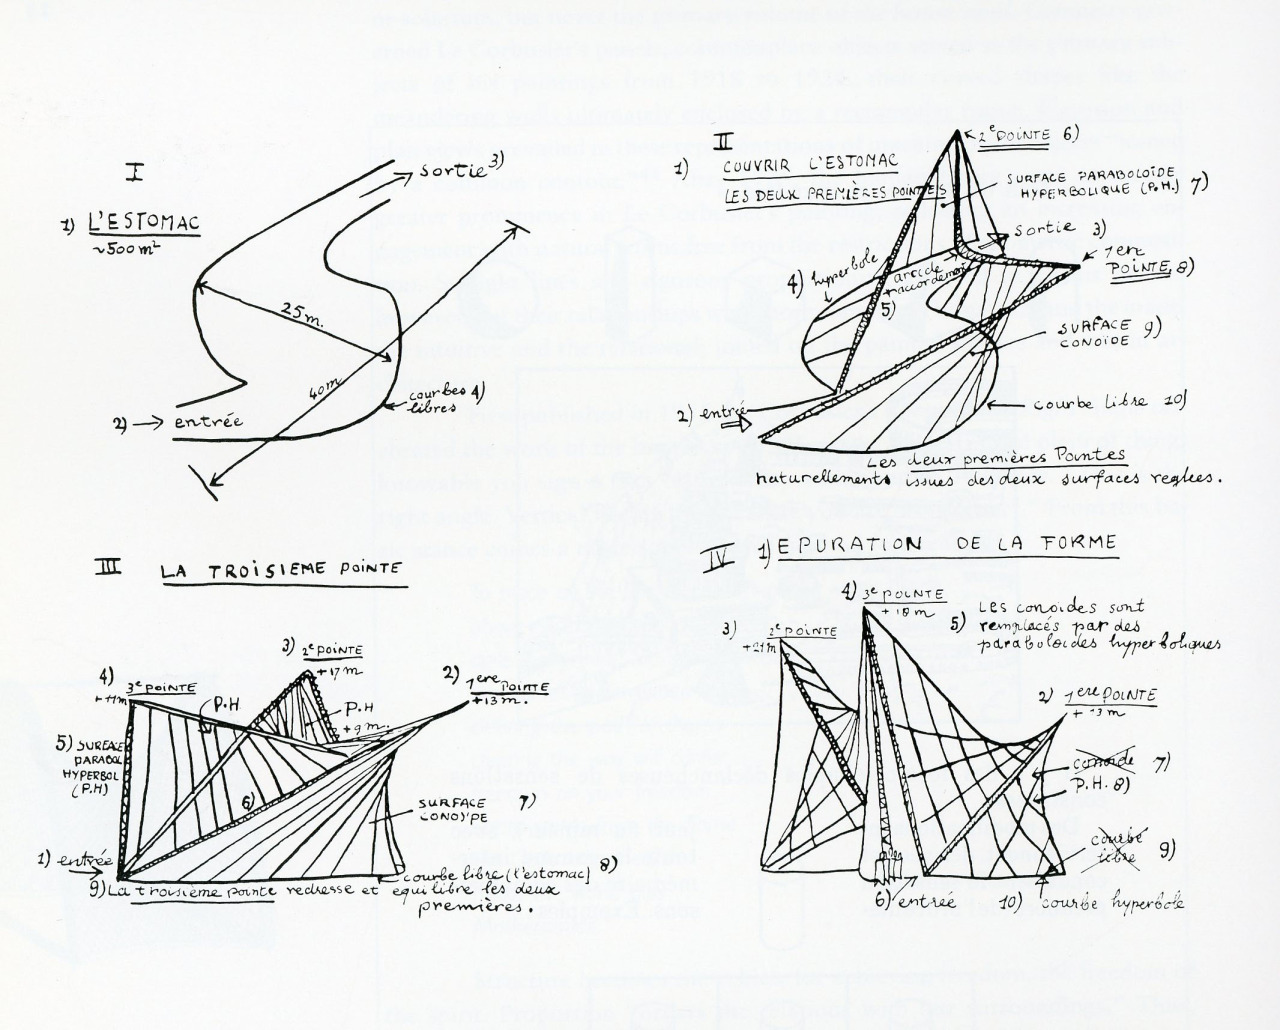
\includegraphics[]{PhilipsDrawings.jpg}
  \caption{Xenakis' early drawings of the Philips Pavilion as
    documented in volume 20 of the \textit{Philips Technical Review}.}
  \label{fig:xenakis-draw}
\end{figure*}

\section{Architecture and Music in Space and Time}
\label{sec:introduction-conclusion}

In \textit{Formalized Music}\cite{xenakis1992formalized}, Xenakis
describes how developments in music theory mimic equivalent
developments in philosophy, mathematics, and the sciences. Plato, for
example, believed that all events transpire as determined by cause and
effect. While Plato and Aristotle both described causality in their
writing, it was not until the 17th century that controlled experiments
and mathematics corroborated the theory.\sidenote[][2mm]{In 1687, Isaac
  Newton published \textit{Philosophi\ae{} Naturalis Principia
    Mathematica} (\textit{Mathematical Principles of Natural
    Philosophy}), in which he compiled the 3 laws of motion that set
  the foundation for the study of \emph{classical mechanics}.}
Similarly, music theory has historically employed causal rules to
describe counterpoint, tonality, and harmonic movement (such as the
natural progression of dominant chord to the tonic).

Causality was largely used to describe physical phenomena until the
19th century when statistical theories in physics began to include
probabilistic notions.\sidenote[][5mm]{The Maxwell-Boltzmann distribution,
  which was first derived by James Clerk Maxwell in 1860, describes
  the probability distribution for the speed of a particle within an
  idealized gas. For more see
  \url{http://plato.stanford.edu/entries/statphys-statmech/}} Xenakis
noticed that more contemporary fields like \emph{probability theory}
generalize and expand on the antecedent theories of causality. Xenakis
thought that music composition should naturally follow the progression
that physics did, with music theory generalizing and expanding on
causal rules that had existed previously. Indeed, starting in the late
19th century and early 20th century, composers like Strauss and
Debussy began to bend the existing rules of music theory, composing
music that branched away from the causal and tonal theories of the
time. With the rise of serialism\sidenote{Serialism is a technique for
  musical composition in which instances of musical elements (such as
  pitch, dynamics, or rhythm), are given numerical values. Sequences
  built from the values are ordered, repeated and manipulated
  throughout the composition.}  and indeterminate music\sidenote{In
  music, indeterminacy refers to the use of chance (such as rolling
  dice or flipping coins) as part of the compositional process.},
composers such as Stockhausen, Boulez, John Cage, Aaron Copland, and
B\'{e}la Bart\'{o}k began to use probability and chance in
composition, the same way that physicists were using probability to
describe the material world. 

To Xenakis' mind, serial music was no less causal than the music it
intended to supersede. He described serial music as embodying
``virtually absolute determinism.''\cite{xenakis1992formalized}
Xenakis saw music theory as a sub-set of mathematics and algebra:
While musicians have a different vocabulary, they also use
mathematical principles to describe and compose music. Because Xenakis
understood mathematics as well as music, he was able to identify how
even in serialism and indeterminate music, composers were only
utilizing a small subset of algebraic theory. In his own music,
Xenakis wanted to generalize and expand the causal framework that
musicians and theorists had been using to compose and understand
music, paralleling similar developments in physics and
mathematics. As a reference to \emph{chance}, or \emph{stochos},
Xenakis coined the term \emph{stochastic music} to describe his
development.

Xenakis' book, \textit{Formalized Music} gives a verbose explanation
of stochastic music. Some authors have interpreted his description
more explicitly. In \textit{Audible Design}, Trevor Wishart describes
the stochastic process used to compose stochastic music as:
\begin{quotation}
  ``A process in which the probabilities of proceeding from one state,
  or set of states, to another, is defined. The temporal evolution of
  the process is therefore governed by a kind of weighted randomness,
  which can be chosen to give anything from an entirely determined
  outcome, to an entirely unpredictable one.''\cite{Wishart1994}
\end{quotation}
% It could be that the lack of a single clear definition by Xenakis is
% the reason that few composers today identify their work as stochastic
% music.

\paragraph{Xenakis' Reflection} In the Spring of 1976, while defending
his doctoral thesis at the University of Paris, Xenakis emphasized the
relevance of seemingly unrelated disciplines to the creative process. A
translation of his defense includes this statement:
\begin{quotation}
  ``The artist-conceptor will have to be knowledgeable and inventive
  in such varied domains as mathematics, logic, physics, chemistry,
  biology, genetics, paleontology (for the evolution of forms), the
  human sciences, and history; in short, a sort of
  \emph{universality}, but one based upon, guided by and oriented
  toward forms and architectures.''\cite{russolo1986art}
\end{quotation}
From Xenakis' drawings we can deduce that he used the same tools,
skills, and philosophy to imagine and conceive both music and
architecture. His approach elevated both forms and blurred the distinction
between the two. Perhaps if we had kept using pen and paper to design
buildings and write music, the reality today would be closer to the
ideal that he imagined. 

As the ideas that inspired Xenakis and other progressive 20th century
composers were taking root in contemporary music, the culture of
artistic form and composition was already beginning the transition
into the digital domain. There is no reason why digital tools cannot
favor stochastic processes to linearity; there is no reason why
digital tools cannot treat music and architecture as equals. However,
even today, software for composing music still favors static pitches
to glissandi; software for architectural design still favors corners
to curves. Most importantly, the software skills that we use to design
and manipulate space, and the skills that we use to compose music,
mutually exclude each other.

This is where the projects described here make a contribution.  By
drawing from music, mathematics, computer science, acoustics, audio
engineering and mixing, sound reinforcement, multimedia production,
and live performance, we can create tools that allow us to
indiscriminately compose with space and sound.

%%% Local Variables:
%%% mode: latex
%%% TeX-master: "CharlesHolbrow_MAS_Thesis"
%%% End:

\chapter{Spatial Domain: \refmod}
\label{ch:ref-mod}

It was Xenakis' goal for the curved surfaces of the Philips Pavilion
to reduce the sonic contribution of sound reflections as much as
possible.\cite{philips1958} He knew that reflections and the resulting
comb filtering could impair intelligibility and localization of music
and sounds. The pavilion was to have hundreds of loudspeakers, and
large concave surfaces like the ones on the inside of the pavilion can
have a focussing effect on acoustic reflections, resulting in severe
filtering and phase cancellations.\cite{Vercammen2008} If Xenakis had
been able to model the reflections and compose them directly into the
piece, what would the tools be like, and how would his architectural
spaces be different? The Xenakis inspired \refmod is an abstract
software tool for experimenting with architectural acoustic lenses. It
is intended more as an experiment for architectural or musical
brainstorming, than as a simulation for analysis of sound
propagation. For example:
\begin{enumerate}
\item It illustrates sound projection in only two dimensions.
\item It is frequency independent. Real sufaces reflect only
  wavelengths much smaller than the size of the
  reflector.\cite{Zhixin2005} 
\item Diffraction is ignored. 
\item Acoustic sounds waves of higher frequencies propagate more
  directionally than lower frequencies. This property is ignored.
% \item The acoustic reflections from, and acoustic diffraction around a
%   real object are dependent on the materials and obstacles behind
%   or adjacent the reflecting surface.\cite{Howard2006} This effect is
%   also not taken modeled by the \refmod.
\end{enumerate}

\section{Implementation}
\label{sec:refmod-implementation}
The \refmod was implemented as a web app using the HTML5
Paper.js\sidenote{\url{http://paperjs.org/}} vector graphics
library.
Try \refmod online at\\
\noindent \url{http://web.media.mit.edu/~holbrow/mas/reflections/}
Click and drag on any black dot to move the object. Black dots
connected by grey lines are handles that re-orient (instead of move)
objects. On reflection surfaces, the handles adjust the angle and
shape of the surface curve. Handles connected to sound sources adjust
the angle and length of the sound beams.
\begin{figure}[h]
% http://web.media.mit.edu/~holbrow/mas/reflections/?q=%7B%22mirrors%22%3A%5B%5B%22Path%22%2C%7B%22applyMatrix%22%3Atrue%2C%22segments%22%3A%5B%5B%5B330%2C60%5D%2C%5B0%2C0%5D%2C%5B-239%2C185%5D%5D%2C%5B319%2C424%5D%5D%2C%22strokeColor%22%3A%5B0%2C0%2C0%5D%2C%22strokeWidth%22%3A2%7D%5D%2C%5B%22Path%22%2C%7B%22applyMatrix%22%3Atrue%2C%22segments%22%3A%5B%5B%5B1035%2C436%5D%2C%5B0%2C0%5D%2C%5B-135%2C113%5D%5D%2C%5B1123%2C534%5D%5D%2C%22strokeColor%22%3A%5B0%2C0%2C0%5D%2C%22strokeWidth%22%3A2%7D%5D%5D%2C%22sounds%22%3A%5B%5B%22Path%22%2C%7B%22applyMatrix%22%3Atrue%2C%22segments%22%3A%5B%5B1047%2C123%5D%2C%5B1048%2C145%5D%5D%2C%22strokeColor%22%3A%5B0.6%2C0.6%2C0.6902%5D%7D%5D%2C%5B%22Path%22%2C%7B%22applyMatrix%22%3Atrue%2C%22segments%22%3A%5B%5B411%2C176%5D%2C%5B480%2C136%5D%5D%2C%22strokeColor%22%3A%5B0.6%2C0.6%2C0.6902%5D%7D%5D%5D%7D
  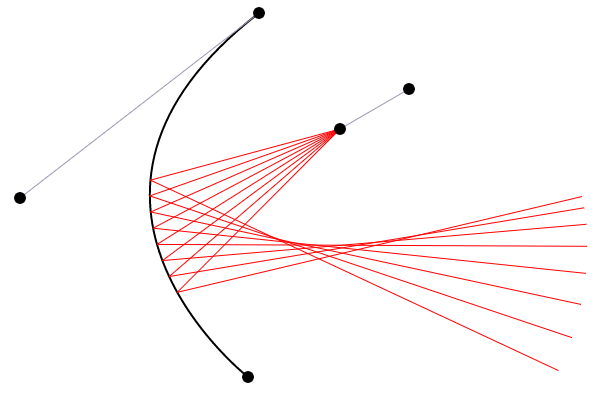
\includegraphics[width=\linewidth]{refmod/1.png}
  \caption[]{\refmod user interface.}
  \label{fig:refmod-simple}
\end{figure}

\section{\refmod Architectural Example}
\label{sec:refmod-user-interf}

Assume we are creating the floor plan for a new architectural space
and accompanying electronic music performance. The music piece
incorporates spatial features in the style of \textit{SOUND=SPACE} by
Rolf Gehlhaar: Our audience moves through the performance space, and
as they move, the sound changes, making the music experience unique to
every visitor. We would like to use acoustic reflections to manipulate
the sound in space, such that at certain points the sound is
focussed on the lister. When we hear an acoustic sound reflection off
a concave surface, the sound can arrive at our ears in two possible
states:
\begin{enumerate}
\item The path of the sound from the source to the reflecting surface
  to our ears is equidistant for each point on the reflecting
  surface. Ignoring any direct sound, the reflection arrives in phase,
  and the surface acts as acoustic amplifier of the reflection.
\item The path of the sound from the source to the reflecting surface
  to our ears is slightly different for each point on the surface. All
  the reflections arrive out of phase with each other.
\end{enumerate}
We can use the \refmod tool to prototype potential layouts and gain some
intuition about where our focal points. The curved black line in the
user interface (figure~\ref{fig:refmod-simple}) represents a
reflective surface. The black dot with emanating red lines represents
a sound source, and the sound propagation.  Each red line emanating
from a sound source is the same length, no matter how many times it
has been reflected. If it is possible to adjust the length of the red
lines such that each one ends at the same spot, it shows that
reflections will arrive at that spot in
phase. Figures~\ref{fig:refmod-bad-focus}
and~\ref{fig:refmod-good-focus} show how we can adjust the curve of a
surface to focus reflections on a point.

\begin{figure}[]
% http://web.media.mit.edu/~holbrow/mas/reflections/?q=%7B%22mirrors%22%3A%5B%5B%22Path%22%2C%7B%22applyMatrix%22%3Atrue%2C%22segments%22%3A%5B%5B%5B513%2C318%5D%2C%5B0%2C0%5D%2C%5B-218%2C117%5D%5D%2C%5B192%2C241%5D%5D%2C%22strokeColor%22%3A%5B0%2C0%2C0%5D%2C%22strokeWidth%22%3A2%7D%5D%2C%5B%22Path%22%2C%7B%22applyMatrix%22%3Atrue%2C%22segments%22%3A%5B%5B%5B1035%2C436%5D%2C%5B0%2C0%5D%2C%5B-135%2C113%5D%5D%2C%5B1123%2C534%5D%5D%2C%22strokeColor%22%3A%5B0%2C0%2C0%5D%2C%22strokeWidth%22%3A2%7D%5D%5D%2C%22sounds%22%3A%5B%5B%22Path%22%2C%7B%22applyMatrix%22%3Atrue%2C%22segments%22%3A%5B%5B1047%2C123%5D%2C%5B1048%2C145%5D%5D%2C%22strokeColor%22%3A%5B0.6%2C0.6%2C0.6902%5D%7D%5D%2C%5B%22Path%22%2C%7B%22applyMatrix%22%3Atrue%2C%22segments%22%3A%5B%5B220%2C202%5D%2C%5B177%2C150%5D%5D%2C%22strokeColor%22%3A%5B0.6%2C0.6%2C0.6902%5D%7D%5D%5D%7D
  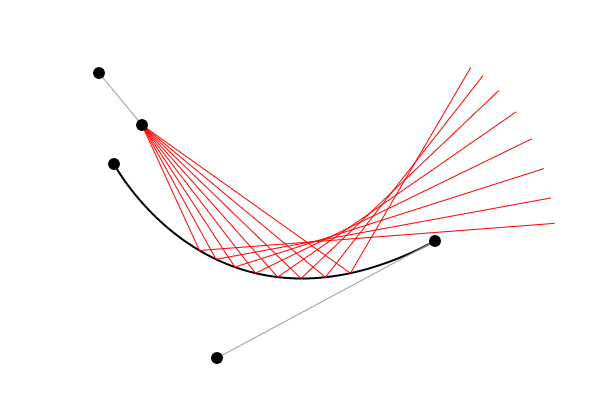
\includegraphics[width=\linewidth]{refmod/out-of-focus.png}
  \caption[]{Reflections from a $30\degree$ loudspeaker arriving out of phase.}
  \label{fig:refmod-bad-focus}
\end{figure}

\begin{figure}[]
%http://web.media.mit.edu/~holbrow/mas/reflections/?q=%7B%22mirrors%22%3A%5B%5B%22Path%22%2C%7B%22applyMatrix%22%3Atrue%2C%22segments%22%3A%5B%5B%5B525%2C318%5D%2C%5B0%2C0%5D%2C%5B-251%2C68%5D%5D%2C%5B180%2C242%5D%5D%2C%22strokeColor%22%3A%5B0%2C0%2C0%5D%2C%22strokeWidth%22%3A2%7D%5D%2C%5B%22Path%22%2C%7B%22applyMatrix%22%3Atrue%2C%22segments%22%3A%5B%5B%5B1035%2C436%5D%2C%5B0%2C0%5D%2C%5B-135%2C113%5D%5D%2C%5B1123%2C534%5D%5D%2C%22strokeColor%22%3A%5B0%2C0%2C0%5D%2C%22strokeWidth%22%3A2%7D%5D%5D%2C%22sounds%22%3A%5B%5B%22Path%22%2C%7B%22applyMatrix%22%3Atrue%2C%22segments%22%3A%5B%5B1047%2C123%5D%2C%5B1048%2C145%5D%5D%2C%22strokeColor%22%3A%5B0.6%2C0.6%2C0.6902%5D%7D%5D%2C%5B%22Path%22%2C%7B%22applyMatrix%22%3Atrue%2C%22segments%22%3A%5B%5B220%2C202%5D%2C%5B179%2C145%5D%5D%2C%22strokeColor%22%3A%5B0.6%2C0.6%2C0.6902%5D%7D%5D%5D%7D
  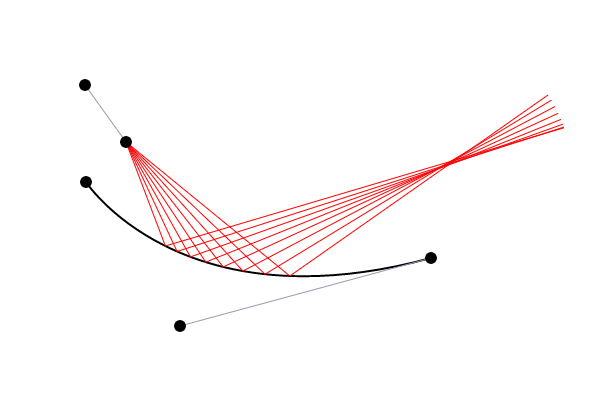
\includegraphics[width=\linewidth]{refmod/in-focus.png}
  \caption[]{By adjusting the curvature of the reflective surface, we
    can focus the audio reflections.}
  \label{fig:refmod-good-focus}
\end{figure}

\begin{figure}[]
%http://web.media.mit.edu/~holbrow/mas/reflections/?q=%7B%22mirrors%22%3A%5B%5B%22Path%22%2C%7B%22applyMatrix%22%3Atrue%2C%22segments%22%3A%5B%5B%5B169%2C416%5D%2C%5B0%2C0%5D%2C%5B405%2C234%5D%5D%2C%5B1178%2C571%5D%5D%2C%22strokeColor%22%3A%5B0%2C0%2C0%5D%2C%22strokeWidth%22%3A2%7D%5D%2C%5B%22Path%22%2C%7B%22applyMatrix%22%3Atrue%2C%22segments%22%3A%5B%5B%5B406%2C321%5D%2C%5B0%2C0%5D%2C%5B135%2C-41%5D%5D%2C%5B651%2C367%5D%5D%2C%22strokeColor%22%3A%5B0%2C0%2C0%5D%2C%22strokeWidth%22%3A2%7D%5D%5D%2C%22sounds%22%3A%5B%5B%22Path%22%2C%7B%22applyMatrix%22%3Atrue%2C%22segments%22%3A%5B%5B431%2C834%5D%2C%5B541%2C796%5D%5D%2C%22strokeColor%22%3A%5B0.6%2C0.6%2C0.6902%5D%7D%5D%2C%5B%22Path%22%2C%7B%22applyMatrix%22%3Atrue%2C%22segments%22%3A%5B%5B278%2C367%5D%2C%5B227%2C266%5D%5D%2C%22strokeColor%22%3A%5B0.6%2C0.6%2C0.6902%5D%7D%5D%5D%7D
  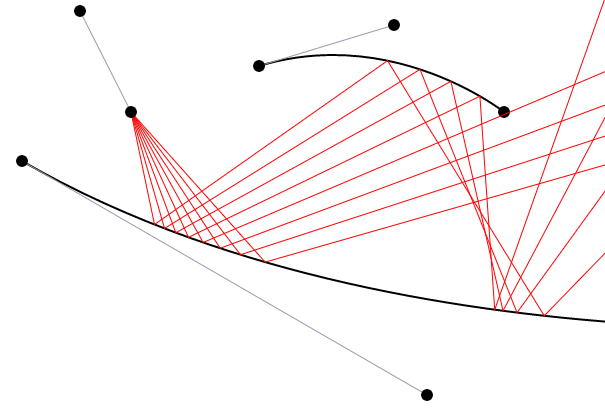
\includegraphics[width=\linewidth]{refmod/music.png}
  \caption[]{A musical composition. The red emanating lines can also
    be thought of as stochastic pitch swarms, similar to those Xenakis
    wrote for Metastasis in 1954 (figure~\ref{fig:metastasis}).}
  \label{fig:refmod-music}
\end{figure}


\begin{figure*}[]
  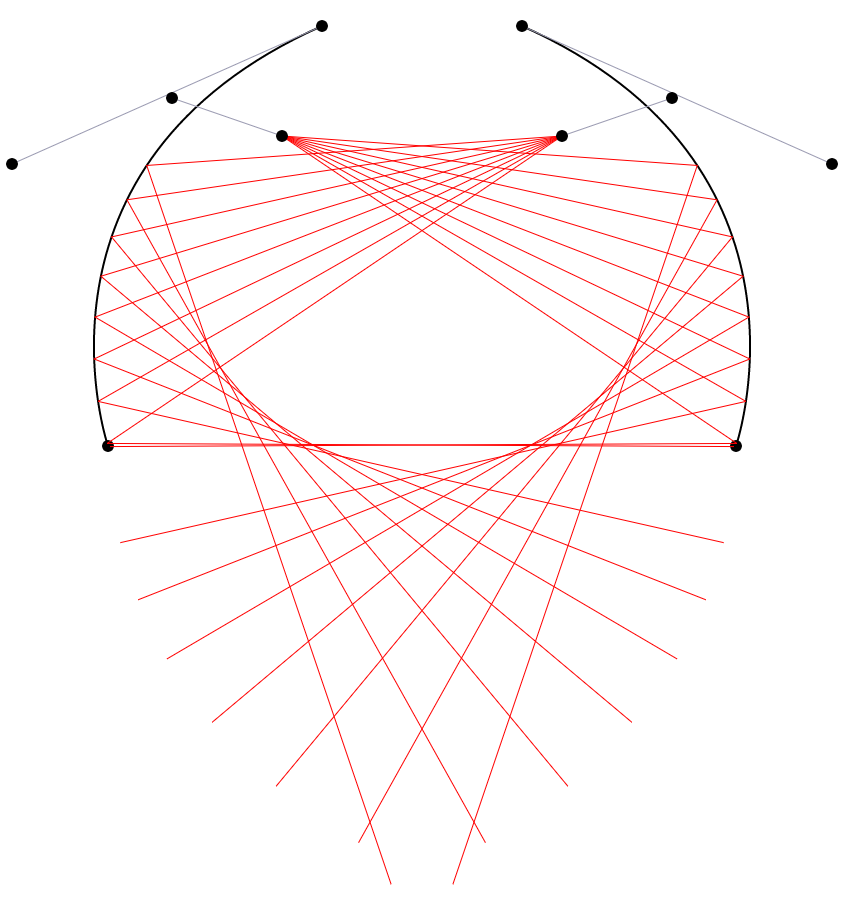
\includegraphics[width=\linewidth]{refmod/refmod.png}
  \caption[]{The \refmod.}
  \label{fig:refmod-full}
\end{figure*}


%%% Local Variables:
%%% mode: latex
%%% TeX-master: "CharlesHolbrow_MAS_Thesis"
%%% End:


\chapter{Time Domain: \polytempic}
\label{ch:polytempic}
In \autoref{ch:introduction} (see figure~\ref{fig:metastasis}) we saw how
Xenakix was using ruled surfaces to create swarms of notes that move
together to create stochastic sonorities. The goal of \polytempic is
to enable composition with swarms of tempo modulations that move in
correlated, cohesive patterns. Music with two or more simultaneous
tempos (polytempic music) is itself not a new concept, and many
examples of polytemic music exist\cite{Greschak2003}. Slightly less
comon is polytempic music where continuous tempo accelerations or
decelerations are defined relative to each other.  This style of music
is well suited to tape music, because tape machines can play
recordings back at variable rates. However, it is difficult to control
the exact point (or phase) when de-synchronized tape becomes
re-aligned. Performative music with simultaneous tempi that accelerate
and decelearate realtive to each other is unusual, but does exist. In
a 1971 interview Composer Steve Reich described how he made the
transition to performative polytempic music after working on his tape
music composition, \textit{Come Out}:
\begin{quotation}
  ``1966 was a very depressing year. I began to feel like a mad
  scientist trapped in a lab: I had discovered the phasing process
  of Come Out and didn't want to turn my back on it, yet I didn't know
  how to do it live, and I was aching to do some instrumental
  music. The way out of the impasse came by just running a tape loop
  of a piano figure and playing the piano against it to see if in fact
  I could do it. I found that I could, not with the perfection of the
  tape recorder, but the imperfections seemed to me to be interesting
  and I sensed that they might be interesting to listen to.''\cite{Nyman2015}
\end{quotation}
Reich's experience illustrates what other composers and performers
have also encountered: It is quite difficult to perform polytempic
music accurately. In \textit{Piano Phase} Reich has two performers
playing the same 12 tone series on the piano. After a set number of
repetitions through the pattern, one performer begins to play slightly
faster until she is exactly one note ahead of the other performer, at
which point both performers play at the same rate for a time. This
process is repeated and iterated on, creating a live \emph{phasing}
effect without the pitch shifting that would occur when phasing analog
tape. If we compare a live performance\cite{Huisman1989} with a
programatic rendering\cite{Chen2014} of \textit{Piano Phase}, we can
hear how the programatic rendering is able to accelearate more
smoothly. The programatic example spends longer on the transitions
where the two parts are out of phase.

\section{Objective}
\label{sec:polytempic-objective}
Steve Reich composed \textit{Piano Phase} for two performers. In his
experimentation, he found that if the music is reasonably simple, two
performers can make synchronized tempo adjustments relative to each
other well enough to yield compelling results. To create stochastic
tempo transitions, our requirements are probably too demainding for
unassisted performers. Our goal is to compose and audition music
where:
\begin{enumerate}
  \item Swarms of an arbitrary number of simultaneous tempi
    coexist. 
  \item Each individual player within the swarm can continously
    accelerate or decelerate individually, but also as a member of a
    cohesive whole. 
  \item Each musical line can converge and diverge at explicit
    points. At each point of convergence the phase of the meter within
    the tempo can be set.
\end{enumerate}
We start by defining a single tempo transition. Consider the following
example shown in figure~\ref{fig:basic-tempo-change}:
\begin{itemize}
\item Assume we have 2 snare drum players. Both begin playing the same
  beat at 90 BPM in common time.
\item One performer gradually accelerates relative to the other. We want
  to define a continous tempo curve such that one drummer accelerates
  to 120 BPM.
\item So far, we can easily accomplish this with a simple linear tempo
  acceleration. However, we want the tempo transition to complete
  exactly when \emph{both} drummers are on a down-beat, so the the
  combined effect is a 3 over 4 rhythmic pattern.
\item We want the accelerating drummer to reach the new tempo after
  exactly 20 beats.
\item We also want the acceleration to complete in exactly 16 beats of
  the original tempo, so the drumer playing a constant tempo, and the
  the accelerating drummer are playing together.
\end{itemize}
\begin{figure*}[h]
  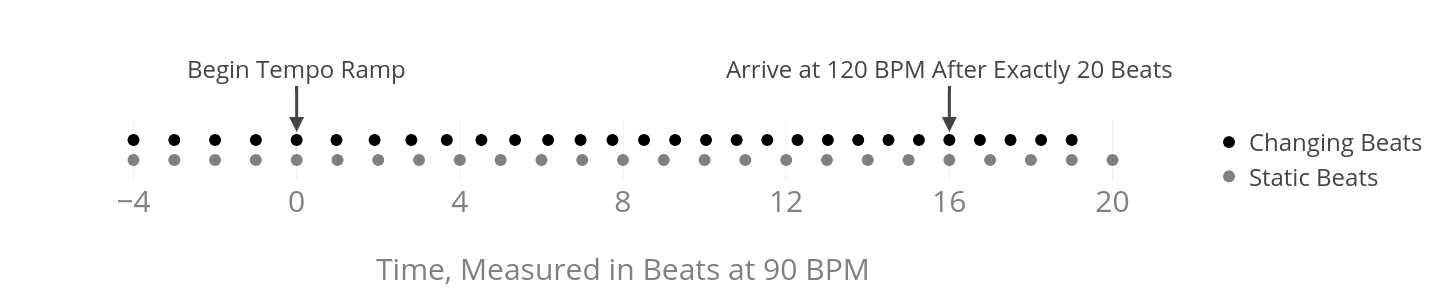
\includegraphics[width=\linewidth]{basic-tempo-transition.png}
  \caption[Tempo Transition]{Tempo Transition from 90 BPM
    to 120 BPM }
  \label{fig:basic-tempo-change}
\end{figure*}

\section{Solution}
\label{sec:polytempic-solution}
We are interested in both the number of beats elapsed in the static
tempo \emph{and} in the changing tempo, and the absolute tempo. Let us
think of the number of beats elapsed as our \emph{position}, and the
tempo as our \emph{rate}, we see how this resembles a physics
problem. If we have a function that describes our tempo (or rate), we
can integrate that function, and the result will tell us our number of
beats elapsed (or position). Given the above considerations, we define
our tempo curve in terms of 5 constants:
\\[5mm]
\begin{fullwidth}
\begin{itemize}
  \item Time $t_0=0$, when the tempo transition begins
  \item A known time, $t_1$, when the tempo transition ends
  \item A known starting tempo, $\dot{x}_0$
  \item A known finishing tempo, $\dot{x}_1$
  \item The number of beats elapsed in the changing tempo between
    $t_0$ and $t_1$, $x_1$
\end{itemize}
\end{fullwidth}
The tension of the tempo curve determines how many beats elapse during
the transition period. The curve is well-defined for some starting
acceleration $a_0$ and finishing acceleration $a_1$, so we define the
curve in terms of linear acceleration. Using Newtonian notation we can
describe our tempo acceleration as:
\begin{equation}
	\label{accel}
    \ddot{x}_1 = a_0 + a_1t_1
\end{equation}
Integrating linear acceleration (\ref{accel}) yields a quadratic
velocity curve. The velocity curve describes the tempo (in beats per
minute)\marginnote{We must specify the same time units for input
  variables like $t_1$ and $\dot{x_1}$. I prefer \textit{minutes} for
  $t_1$ and \textit{beats per minute} for $\dot{x_1}$ over
  \textit{seconds} and \textit{beats per second}} with respect to
time.
\begin{equation}
	\label{bpm}
    \dot{x}_1 = \dot{x}_0 + a_0t_1 + \frac{a_1t_1^2}{2}
\end{equation}
Integrating velocity (\ref{bpm}) gives us a function describing the number 
of beats elapsed with respect to time.
\begin{equation}
	\label{beats-elapsed}
	x_1 = x_0 + \dot{x}_0t_1 + \frac{a_0t_1^2}{2} + \frac{a_1t_1^3}{6}
\end{equation}
With equations (\ref{bpm}) and (\ref{beats-elapsed}), we can solve for our 
two unknowns, $a_0$ and $a_1$. First we solve both equations for $a_1$:
\begin{displaymath}
    \label{a1-solution}
    a_1=
    \frac{-2}{t_1^2}(\dot{x}_0-\dot{x}_1 + a_0t_1)=
    \frac{-6}{t_1^3}(\dot{x}_0-x_1 + \frac{a_0t_1^2}{2})
\end{displaymath}
Assuming $t_1 \neq 0$, we solve this system of equations for $a_0$:
\begin{equation}
	\label{a0-result}
	a_0=\frac{6x_1-2t_1(\dot{x}_1+2\dot{x}_0)}{t_1^2}
\end{equation}
Evaluating (\ref{a0-result}) with our constants gives us our starting
acceleration. Once we have $a_0$ we can solve (\ref{bpm}) for $a_1$, and 
evaluate (\ref{bpm}) with $a_1$ and $a_0$ to describe our changing tempo 
with respect to time.

\section{Implementation}
\label{sec:polytempic-implementation}

Bryn Bliska Tide

\begin{figure*}[h]
  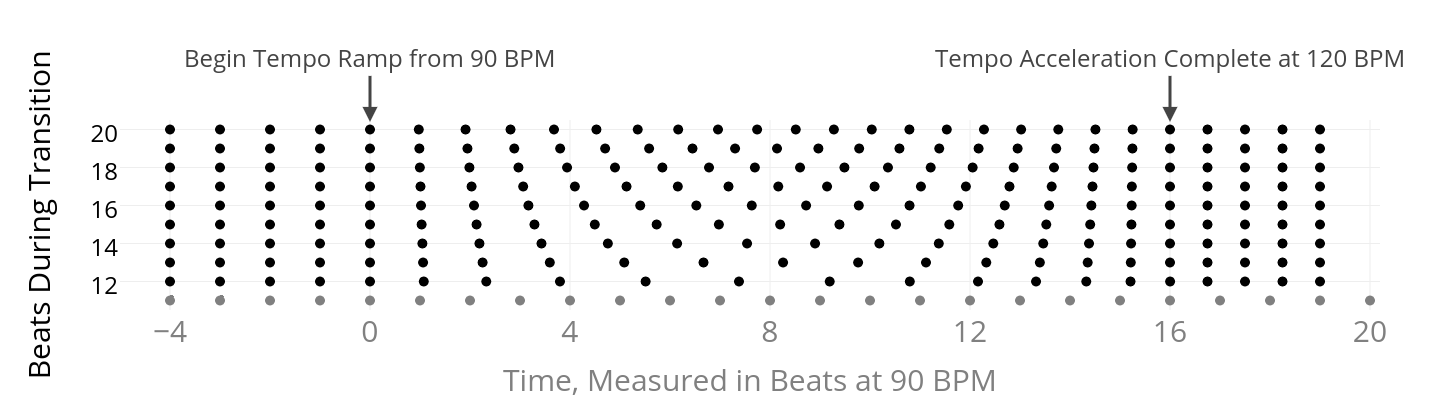
\includegraphics[width=\linewidth]{stochastic-tempi.png}
  \caption{Stochastic Tempo Transition from 90bpm to 120bpm}
  \label{fig:metastasis}
\end{figure*}


\section{Polytempic Music and Polymetric Music}
\label{sec:polytempic-vs-polymetric}
It is easy to confuse poly tempic music with polymetric music.  Pieces
where multiple meter
Other notable composers
of the time include John Cage, who wrote wrote what he called, Chance
Music, and Stockhausen, Boulez and Berio who wrote aleatoric music.



Eliot Carter: Polymetric Modulation. 
Steve Reich: Piano Phase
Paper: realtime representation of 
Paper: Stochos: Software for Real-Time Synthesis of Stochastic Music

John Cage: Chance Music
Karlheinz Stockhausen, Pierre Boulez, Luciano Berio: Aleatoric music

\section{Contribution}
\label{sec:polytempic-contribution}

and finishes the tempo transition slightly different tempos.

To audition stochastic tempo transitions, we can create software tools
that promt musicians with visual cues or aural cues, 
More flexible Digital Audio Workstations (DAWs) like Reaper and
Digital Performer include workarounds for auditioning simultaneous
tempo. 

For example we 

Xenakis was among a group of
20th century composers who were searching for ways to push the
boundaries of established music composition.


%%% Local Variables:
%%% mode: latex
%%% TeX-master: "CharlesHolbrow_MAS_Thesis"
%%% End:

\chapter{The Hypercompressor}
\label{ch:hypercompressor}

The motivation for Hypercompression came during the development of
Vocal Vibrations, an interactive music installation about the human
voice and about engaging the public in singing.\cite{Holbrow2014} The
project featured a Music Concr\`{e}te composition, \textit{The Chapel}
by Tod Machover, which was mixed in a 10 channel surround sound
format and played throughout the installation. During the mixing
process, I noticed an important surround sound tool missing from my
mixing workflow. When mixing in mono or stereo, audio
compression\marginnote{Unless noted otherwise, ``compression'' is used
  in this thesis to describe dynamic range compression, as opposed to
  data compression.} lets us meticulously shape and balance sounds in
time. I found myself wishing I could shape and position sounds in
space just as easily.

\section{Building on the Compression Paradigm}
The design, implementation, and use of traditional dynamic range
compression is well documented in the
literature,\cite[]{Giannoulis2012,Case2007,Deruty2014} so we will
describe dynamic range compression only as much as is needed to
explain the foundation for \thesis. Imagine we are mixing a vocal pop
performance, and during the verse our vocalist is singing moderately
loud, or \textit{mezzo-forte}. At the beginning of the chorus, our
singer wants a full and powerful sound, so she adjusts the dynamic to
very loud, or \textit{fortissimo}. However, the new louder dynamic
interrupts the balance between the vocals and the other instruments in
our mix. We like the powerful sound of our singer's
\textit{fortissimo} performance, but our balance would be improved if
we had the volume of a \textit{forte} performance instead. One option
is to manually turn down the vocalist during the chorus, which in some
cases this is the best solution. When we want more precise control, we
can use a compressor.

\subsection{Traditional Compression}
\label{sec:trad-compr}
A compressor is essentially an automated dynamic volume control.  Most
compressors include at least four basic parameters in the user
interface that allow us to customize its behavior: \textit{threshold},
\textit{ratio}, \textit{attack time}, and \textit{release time}.  We
can send our vocalist's audio signal through a compressor, and
whenever her voice exceeds the gain level set by our threshold
parameter, the signal is automatically attenuated. As the input signal
further exceeds the threshold level, the output is further attenuated
relative to the input signal. The ratio parameter determines the
relationship between the input level and output level as shown in
figure~\ref{fig:comp-ratio}.

\begin{marginfigure}
  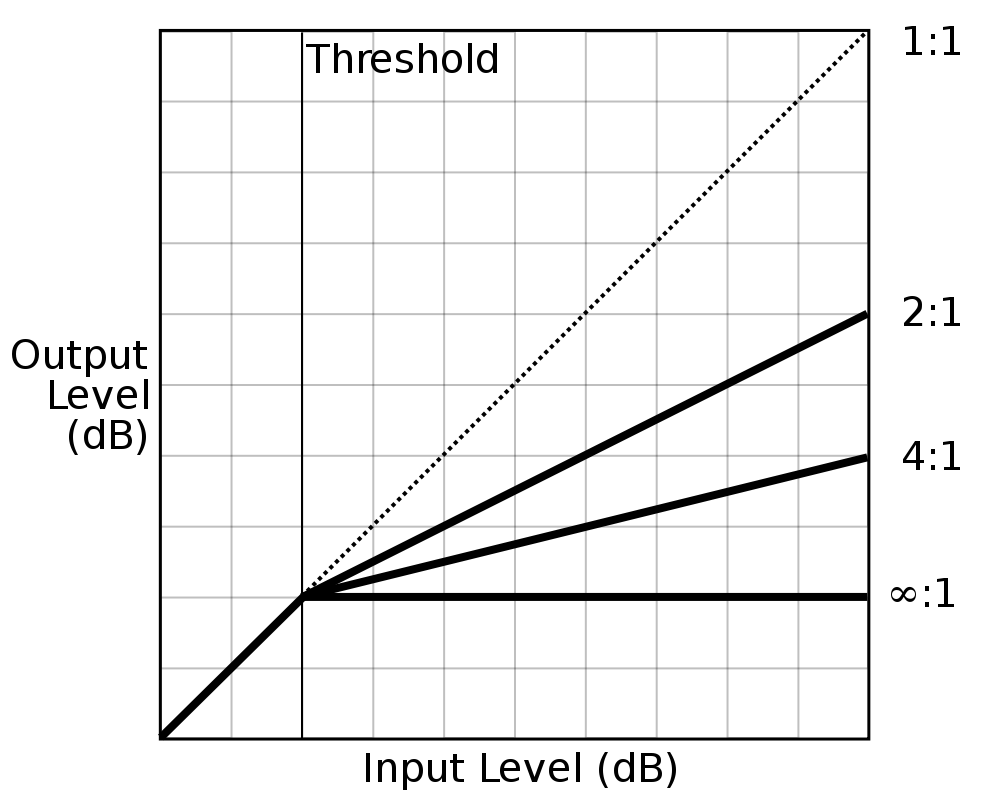
\includegraphics[]{CompressionRatio.png}
  \caption{``Compression ratio'' by Iain Fergusson. Licensed under
     Public Domain via Wikimedia Commons 
     \url{https://commons.wikimedia.org/wiki/File:Compression_ratio.svg\#/media/File:Compression_ratio.svg}
   }
  \label{fig:comp-ratio}
\end{marginfigure}

Threshold and ratio settings are essential for controlling dynamic
range, but the power and creative flexibility of the compressor comes
with the attack time and release time parameters. These parameters
determine the speed at which the compressor attenuates (attack time)
and disengages (release time) when the input signal exceeds the
threshold. By adjusting the attack and release times, we can change
the temporal focus of the compressor.
\begin{itemize}
\item Perhaps we want the compressor to engage or disengage at the
  time scale of a musical phrase. We could set our attack time long
  enough to let transients through without engaging the compressor
  significantly (try 20 milliseconds). If our release time is quite
  long (try 300 milliseconds), and we set our threshold and ratio
  carefully, we might be able to convince the compressor to smooth
  musical phrases.
\item If we want our compressor to focus on syllables instead of
  phrases, we can shorten our attack and release times (try 10
  milliseconds and 40 milliseconds respectively). When the compressor
  engages and disengages at each syllable, it imparts a different
  quality (sometimes described as ``punch'').
\item If we reduce our attack and release parameters enough, we can
  instruct our compressor to engage and disengage at the time scale of
  an audio waveform, compressing individual cycles. This will distort
  an audio signal, adding odd order harmonics,\sidenote{Not every
    compressor model can react quickly enough to distort a
    waveform. The Dbx 160 and Teletronix LA2A are known to be fast
    enough to distort.} and imparting an entirely different quality.
\end{itemize}
The attack and release times listed here are a rough guide only.  The
exact function of these parameters varies from one model of compressor
to another, and results also depend on the audio input material and
on the threshold and ratio settings. The results of audio
compression can sometimes be characterized better by a feeling than a
formula.

\begin{figure*}
  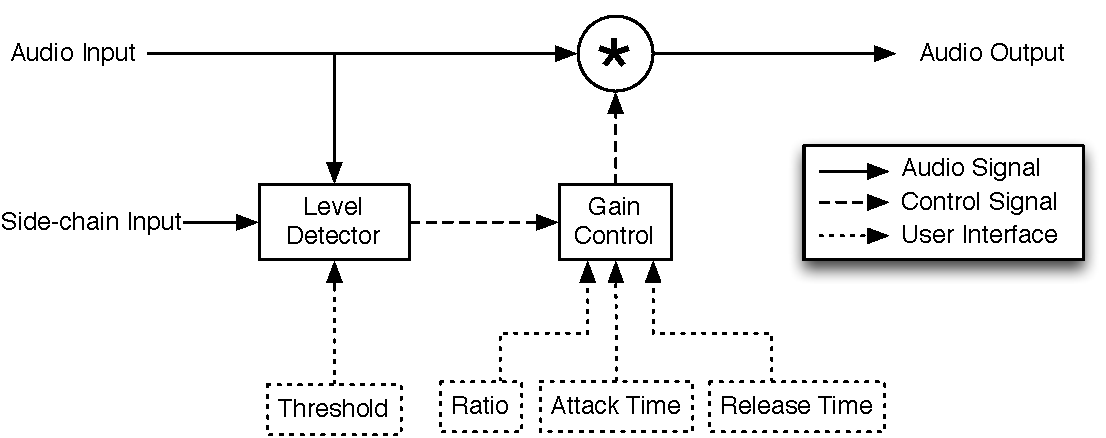
\includegraphics[width=\linewidth]{hypercomp/SimpleCompressor.pdf}
  \caption{Block diagram of a simple traditional dynamic range
    compressor.}
  \label{fig:comp-block}
\end{figure*}

\subsection{Side-Chain Compression}
\label{sec:side-chain-compr}
Compressors often have an additional operational mode that is the
primary inspiration for Hypercompression. We know that compressors
automatically reduce the gain of a signal that exceeds a given
threshold. Some compressors allow us to attenuate the level of a
signal when a \emph{different} signal exceeds the threshold
level. Models that suports side-chain compression have a second audio
input. When we switch the compressor into side-chain mode, the
compressor attenuates the first signal only when the second signal
exceeds the threshold.

Side-chain compression is often used to moderate the balance of kick
drum and bass guitar. If the bass guitar is briefly attenuated just
enough just the right amount each time the kick drum hits, we can set
the kick and bass guitar at exactly the gain levels we want without
one masking the other. Because the bass guitar is only briefly
attenuated, it will not be perceived as any quieter.

In this example we use the kick drum to create a gain envelope for our
bass guitar. The kick \emph{pushes} the bass to make room for
itself. The attack time and release time parameters give control over
this behavior in the temporal domain. The next step is to
expand this model to add control in the spatial domain.

\section{Ambisonics}
\label{sec:ambisonics}
Ambisonics is a technique for encoding and decoding three-dimensional
surround sound audio.\cite[-15mm]{Gerzon1973,Gerzon1985} Ambisonic
audio differs from other surround sound formats like $5.1$ and $7.1$
in that it does not depend on a particular speaker configuration. An
ambisonic recording can be decoded on any surround sound speaker
configuration without disarranging the spatial contents of the audio
recording.

Imagine we use an omnidirectional microphone to record an acoustic
instrument at a sample rate of 44.1 kHz. We sample and record 44100
samples every second that represent the air pressure at the microphone
capsule during the recording. Our omni-directional microphone is
designed to treat sound arriving from all angles equally. The
omnidirectional microphone sums together sounds arriving from all
angles and the acoustic directional information is lost.

If we want to encode, decode, transmit, or play audio that preserves
full sphere 360 degree information, ambisonics offers a solution.
Ambisonic audio uses \textit{spherical harmonics} to encode surround
sound audio that preserves the direction-of-arrival information that
discrete channel recordings (such as mono and stereo) cannot fully
capture.

\subsection{Spherical Harmonics}
\label{sec:spherical-harmonics}
We know that we can construct any monophonic audio waveform by summing
a (possibly infinite) number of harmonic sine waves (Fourier
series).\sidenote{An excellent description of the transformation between
  the time domain and frequency domain can be found at
  \url{http://betterexplained.com/articles/an-interactive-guide-to-the-fourier-transform/}}
For example, by summing odd \textit{order} sine harmonics at a given
frequency $f$, $(1f, 3f, 5f, 7f, \ldots )$, we generate a square wave
with fundamental frequency $f$. As the order increases, so does the
temporal resolution of our square wave.

By summing sinusoidal harmonics, we can generate any continuous
waveform defined in two dimensions (one input parameter and one
output). Similarly, by summing \emph{spherical harmonics}, we can
generate any continuous shape defined over the surface of a
three-dimensional sphere (two input parameters, or polar angles, one
output). Where a traditional monophonic audio encoding might save one
sample 44100 times per second, an ambisonic encoding would save one
sample \emph{for each spherical harmonic} 44100 times per second. This
way we capture a three-dimensional sound image at each audio sample.
The number of spherical harmonics we encode is determined by our
\textit{ambisonic order}. As our ambisonic order increases, so does
the angular resolution of our result on the surface of the sphere.

\subsection{Spherical Harmonic Definition}
For encoding and decoding ambisonics, the convention is to use the
real portion of spherical harmonics as defined in
equation~\ref{eq:spherical}, where:
\begin{itemize}
\item $Y_{n}^{m}(\varphi,\vartheta)$ is a spherical harmonic that
is:\marginnote{Some literature on spherical harmonics swaps the names
  of \textit{order} and \textit{degree}. In this thesis we use
  $Y_{order}^{degree}$. In literature where $Y_{degree}^{order}$ is
  used, the function of the subscript and superscript remain
  unchanged; only the names are inconsistent.}
\begin{itemize}
\item of order, $n$
\item of degree, $m$
\item defined over polar angles $(\varphi, \vartheta)$
\end{itemize}
\item $N_n^{|m|}$ is a normalization factor.\sidenote{In ambisonic
    literature (and software), there are multiple incompatible
    conventions for the normalization of spherical harmonics. The
    Hypercompressor uses the \textit{Furse-Malham} (FuMa)
    normalization convention.}
\item $P_n^{|m|}$ is the associated Legendre function of order $n$
  and degree $m$.
\end{itemize}
\begin{equation}
Y_{n}^{m}(\varphi,\vartheta)=N_n^{|m|}P_n^{|m|}(\sin{\vartheta})
\begin{cases}\label{eq:spherical}
\sin{|m|\varphi},&  \text{for $m<0$}\\  
\cos{|m|\varphi},& \text{for $m\geq 0$}\\
\end{cases}
\end{equation}
Given equation~\ref{eq:spherical}, we can define an ambisonic
audio recording as:
\begin{equation}
f(\varphi,\vartheta,t)=\sum\limits_{n=0}^N\sum\limits_{m=-n}^nY_n^m(\varphi,\vartheta)\phi_{nm}(t)
\label{eq:ambisonics}
\end{equation}
Where:
\begin{itemize}
\item $\varphi$ and $\vartheta$ describe the polar angle of sound
  arrival in two dimensions.\sidenote{Note that ambisonics uses polar
    angles to describe the angle of arrival of sound. These are
    similar to spherical coordinates, minus the inclusion of
    \textit{radial distance}. Distance is not part of the ambisonic
    specification.}
\item $t$ is time
\item $\phi_{nm}(t)$ are our \textit{expansion coefficients}, described
  below.
\end{itemize}
\begin{figure}[h]
  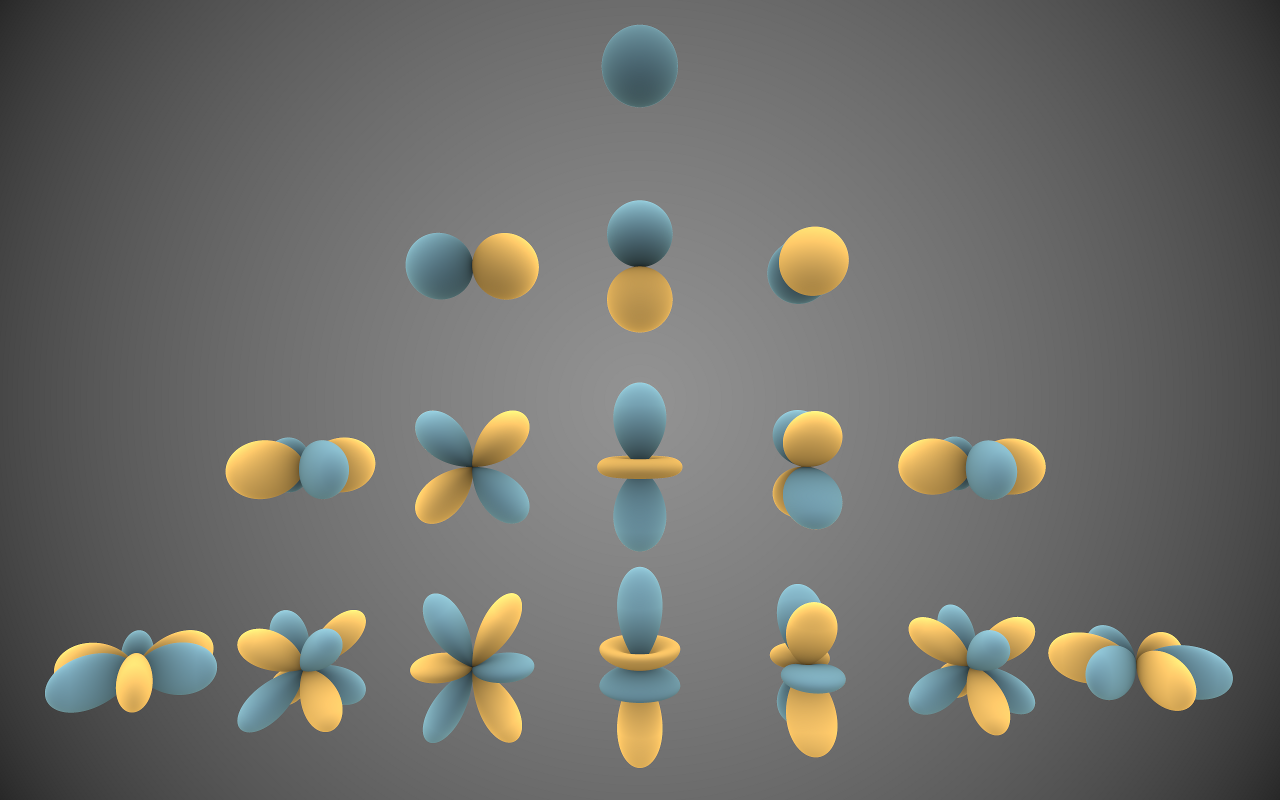
\includegraphics[width=\linewidth]{SphericalHarmonics.png}
  \caption{Spherical harmonics $0$th order (top row) through $3$rd
    order (bottom row). This for image shows the output of
    $Y_{n}^{m}(\varphi,\vartheta)$ for $n=0,n=1,n=2,$and $n=3$. The
    distance of the surface from the origin shows the value at that
    angle. Darker blue regions are positive, while lighter yellow
    regions are negative. Image credit: Ingo Quilez, licensed under
    \textit{Creative Commons Attribution-Share Alike 3.0 Unported}.}
  \label{fig:spherical-harmonics}
\end{figure}

\subsection{Spherical Harmonic Expansion Coefficients}
\label{sec:spher-harm-expans}
In our monophonic recording example, we save just one digital sample
44100 times per second, with each saved value representing the air
pressure at a point in time. We know that by summing the correct
combination of spherical harmonics, we can describe any continuous
function over the surface of a sphere. Instead of sampling air
pressure directly, we sample a coefficient describing the weighting of
each spherical harmonic 44100 times per second. The resulting sphere
encodes the pressure including the direction of arrival
information. The weighting coefficients or \textit{expansion
  coefficients} are recorded in our audio file instead of values
representing air pressure directly. Now, by summing together our
weighted spherical harmonics, we can reconstruct the fluctuations in
pressure including the angle of arrival information. We can recall
this snapshot of information at our 44.1 kHz audio sample rate.

\subsection{Ambisonic Encoding}
\label{sec:usage}
There are two ways to create an ambisonic recording. First, we can use
a soundfield microphone to record an acoustic soundfield. Soundfield
microphones like the one developed by Calrec Audio can capture angle
of arrival information with the spatial resolution of first order
ambisonics.\cite[-1in]{Ferrar1979} Alternatively, we can algorithmically
encode pre-recorded sources, creating virtual sources in an
ambisonic bus.\cite[-0.4in]{Malham1995}

\section{Ambisonic Conventions used for Hypercompression}
\label{sec:ambis-conv-used}
This thesis follows ambisonic convention for describing axis of
rotation. The x-axis points forward, the y-axis point left, and the
z-axis points up. Polar angles are used to describe orientation with
$0\degree$ azimuth being forward, and increasing as we move to the
left. $0\degree$ elevation also points forward, and increases as we
move upward, with $90\degree$ being strait up along the z-axis. When
working with ambisonics, multiple inconpatible conventions exist for
ordering and normalizing spherical harmonics.\cite{Nachbar2011} The
Hypercompressor uses \textit{Furse-Malham} normaliation
(FuMa)\cite{Malham2003}, and first order ambionics with
\textit{B-format}\cite{Hollerweger2008} channel ordering. B-format
ordering labels the four first-order ambisonic channels as W, X, Y,
and Z, with W being the spherical harmonic of order zero and degree zero,
and X, Y, and Z being the ressure gradient components along their
respective axes. 

\section{Hypercompressor Design}
\label{sec:hypercomp-design}
\begin{figure*}
  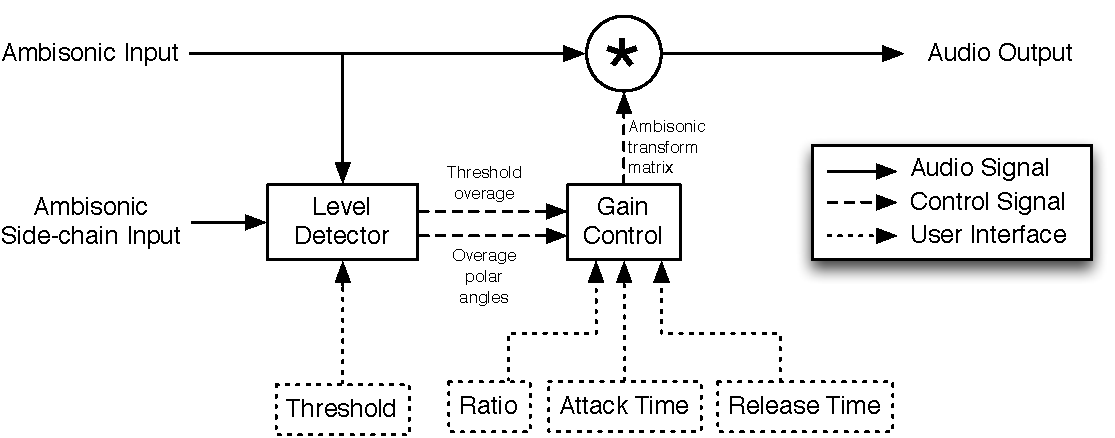
\includegraphics[width=\linewidth]{hypercomp/AmbisonicCompressor.pdf}
  \caption{Block diagram of the Hypercompressor.}
  \label{fig:hypercomp-block}
\end{figure*}
\noindent The Hypercompressor (or ambisonic compressor) combines the traditional
model of compression with the surround sound capability of
ambisonics. Given ambisonic input, and an optional ambisonic
side-chain input, the ambisonic compressor is intended to process our
input material in one of two modes:
\begin{enumerate}
\item Standard mode: We set a compression threshold, similar to on a
  traditional compressor. When a region in our surround sound input
  material exceeds the set threshold, the compressor engages and
  attenuates only that region.
\item Side-chain mode: This mode takes advantage of a second ambisonic
  input to our signal processor. When the gain of spatial region in
  our secondary input exceeds our threshold, we attenuate that same
  region in the the main input, and output the results.
\end{enumerate}
In both modes, our ambisonic compressor must attenuate and release
attenuation according to the attack time and release time
parameters. The block diagram for our new hypercompressor
(figure~\ref{fig:hypercomp-block}) can remain largely unchanged from
the the block diagram for our traditional compressor in
figure~\ref{fig:comp-block}. The most important changes are:
\begin{itemize}
\item Our audio signals must be updated to handle encoded
  ambisonics. This is as simple as increasing the number of channels
  on each solid black connection in figure~\ref{fig:comp-block}. The
  hypercompressor works with first order ambisonics, so every audio
  path must carry four audio channels.
\item On a traditional compressor, the level detector only needs to
  detect the difference between the gain of the input signal and the
  gain specified by the threshold parameter. Our ambisonic level detector
  needs to decode the incoming signals and identify both a threshold
  overage and the region where the overage occurred.
\item Our gain control module needs to listen to the input coming from
  the level detector module and be able to attenuate the specific
  regions that exceed our threshold parameter.
\end{itemize}

\subsection{Level Detection Module}
\label{sec:an-accurate-level}
In \textit{Spatial Transformations for the Alteration of Ambisonic
  Recordings}, Matthias Kronlachner describes
one approach for making a visual ambisonic level meter:\cite{Kronlachner2014} 
\begin{enumerate}
\item Choose a series of discrete points distributed on the surface of
  a sphere. Ideally the points are equally distributed, so the
  vertices of platonic solid shapes like the dodecahedron (12-sided
  polyhedron) and icosahedron (20-sided polyhedron,
  figure~\ref{fig:icosahedron}) work well. For spatial accuracy,
  Kronlachner recommends a spherical $t$-design with 240 points
  described by Hardin and Sloane.\cite{Hardin1996}
\item Evaluate each spherical harmonic at every point chosen. Cache
  the results in a matrix. 
\item With the cached spherical harmonics, it is then possible to
  calculate the RMS and peak values more efficiently at the audio
  rate.
\item A level meter does not need to refresh the display at the audio
  sample rate, so it is acceptable to interpolate between the points
  on the sphere and update the graphical representation at the
  control rate, which could be as slow as 30 Hz (approximately every
  33 milliseconds).
\end{enumerate}
\begin{marginfigure}
  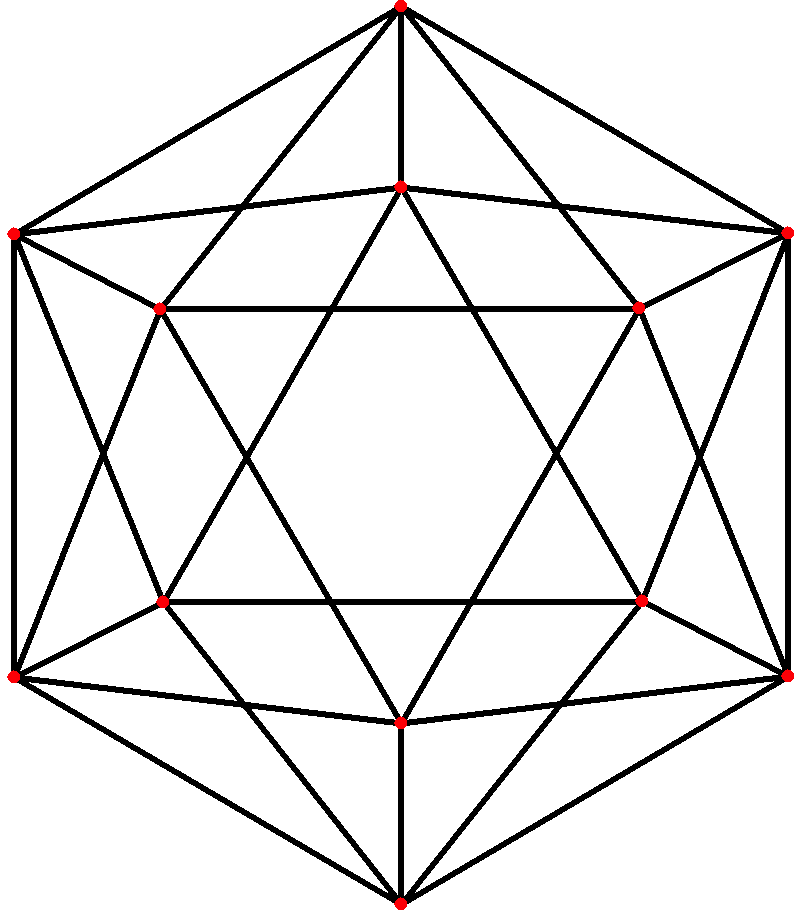
\includegraphics{hypercomp/Icosahedron.png}
  \caption{An icosahedron.}
  \label{fig:icosahedron}
\end{marginfigure}
A similar approach can be used to make an ambisonic level
detector. However, a compressor needs to react much quicker than a
level meter. The compressor cannot even \emph{begin} to engage until
the level meter has responded, and attack times faster than 33
milliseconds are common in conventional compression. Every point on
the sphere requires a buffer to calculate the RMS. We also need to
decode ambisonics at the audio sample rate and keep track of peak
values. Ideally we would also interpolate between the points.

\subsection{An Efficient Level Detection Module}
\label{sec:hyperc-level-detect}
The Hypercompressor needs to detect the level of our ambisonic input
material and identify (as quickly as possible) when and where the
signal exceeds the compressor threshold. In the interest of
computational efficiency, the first level detector I wrote attempted
to extract overage information with minimal ambisonic decoding and
signal processing.
\begin{enumerate}
\item To accurately play a first order ambisonic encoding, we need a
  minimum of 6 speakers placed around the listener. In this level
  detector, we calculate the root mean square (RMS) average at the
  center of 6 lobes corresponding to the first order spherical
  harmonics: front, rear, left, right, top, and bottom.
\item Calculate a map of the influence of each lobe on the surround
  image\TODO{Clean}
  (figures~\ref{fig:hypercomp-mathematica},~\ref{fig:hypercomp-inf-maps}). For
  example, pan a monophonic sound directly forward in an ambisonic
  mix, cache an image of the resulting sound sphere. Save one image
  for each of the 6 lobes.
\item We have 6 images, each representing one of the 6 lobes of our
  first order ambisonic spherical harmonics. In step 1, we calculated
  the RMS level at each of the corresponding points on our surround
  sphere. Use the 6 RMS levels to weight each of our 6 maps. The sum
  of the weighted maps shows the gain distributed across our ambisonic
  sphere.
\end{enumerate}

\begin{figure}[]
  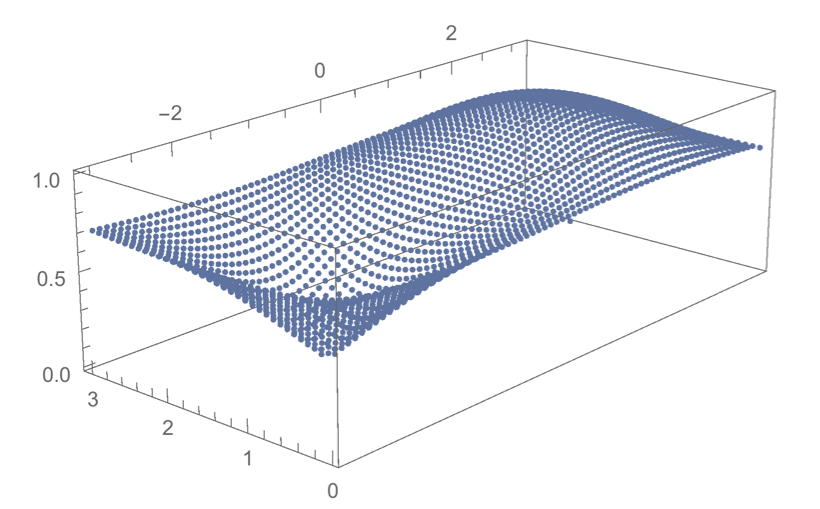
\includegraphics[width=\linewidth]{hypercomp/AmbisonicFieldAngle.png}
  \caption{Calculating the cylindrical projection of single ambisonic panned
    source in the Wolfram Mathematica software package}
  \label{fig:hypercomp-mathematica}
\end{figure}

\begin{figure}[]
 
\includegraphics[width=3.5cm]{hypercomp/left_x72.png}
 
\includegraphics[width=3.5cm]{hypercomp/above_x72.png}
 
\includegraphics[width=3.5cm]{hypercomp/front_x72.png}
 % 
\includegraphics[width=3.5cm]{hypercomp/right_x72.png}
 % 
\includegraphics[width=3.5cm]{hypercomp/below_x72.png}
 % 
\includegraphics[width=3.5cm]{hypercomp/rear_x72.png}
  \caption{Influence maps of 3 first-order spherical harmonics: left, top, and
    front. Pure white is $-0$~dBFS black is -inf~dBFS. Cylindrical projection.}
  \label{fig:hypercomp-inf-maps}
\end{figure}

\paragraph{Results:}If the input to the level detector is encoded as
an ambisonic plane wave, this level detector does yield accurate
results.  In the more common case, when our ambisonic input material
contains multiple sources that are each ambisonically panned to
different positions, this interpolation technique does not accurately
calculate the RMS at any angle. In simple cases, where we can be sure
our input material is appropriate, the technique described here might
be useful, but in most cases, a different approach will be more
effective.

\begin{figure}[h]
%  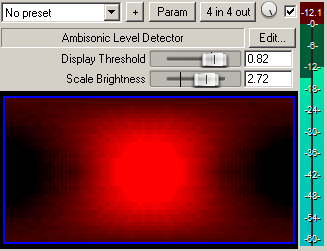
\includegraphics{hypercomp/LevelDetect_front.png}
  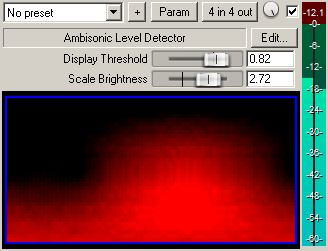
\includegraphics{hypercomp/LevelDetect_45_down.png}
  \caption{The Hypercompressor visualizer written for the efficient
    ambisonic level detector. The surround sphere is projected to a
    cylinder and unwrapped on the flat surface. In this image, a
    monophonic source is panned slightly down and to the right
    ($-45\degree$ azimuth, $-45\degree$ elevation).}
  \label{fig:hypercomp-inf-map-angle}
\end{figure}

\subsection{Ambisonic Gain Control Module}
\label{sec:ambis-gain-contr}
The spherical harmonics defined in equation~\ref{eq:ambisonics} form a
set of orthogonal basis functions. If we define a sequence for our
spherical harmonics and spherical harmonic expansion coefficients, we
can treat the expansion coefficients as vectors and perform matrix
operations on them that rotate, warp, and re-orient our
three-dimensional surround sound image.\cite{Pomberger2011} The
ability to mathematically warp and manipulate our surround sound image
makes ambisonics the perfect choice for implementing a surround sound
compressor.

\paragraph{The Focus Transform} One transform that lets us attenuate a
region of the surround sound sphere is the \textit{focus} transform
distributed as part of the open source Ambisonic Toolkit
(ATK)\sidenote{\url{http://www.ambisonictoolkit.net/}} This transform
is intended to focus on transform is intended to focus on the 
\cite{Anderson2009}
\begin{fullwidth}
\[ \left( \begin{array}{cccc}
\frac{1}{1 + \sin|w|} & 
\frac{1}{\sqrt{2}} \frac{\sin(w)}{1 + \sin|w|}  & 
0 &
0 \\
\sqrt{2}\frac{sin(w)}{1 + \sin|w|} & % LG1
\frac{1}{1 + \sin|w|} &                    % LG0
0 & 
0 \\
0 & 
0 &
\frac{\cos(w)}{1 + \sin(w)} &
0 \\
0 &
0 &
0 &
\frac{\cos(w)}{1 + \sin|w|} 
\end{array} \right)
\]
\end{fullwidth}
%%% Local Variables:
%%% mode: latex
%%% TeX-master: "CharlesHolbrow_MAS_Thesis"
%%% End:

\clearpage
\chapter{\textit{De L'Exp\'{e}rience}}
\label{ch:experience}

\textit{De L'Exp\'{e}rience} is a composition by Tod Machover in in
eight sections for narrator, organ, and electronics. The piece was
commissioned by the \textit{Orchestre Symphonique de Montr\`{e}al}
(OSM), and premiered at the \textit{Maison Symphonique de
  Montr\'{e}al} on May 16th, 2015. The text for the piece was taken
from the writings of Michel de Montaigne, the 16th century philosopher
known for popularizing the essay form.  Performers include Jean-Willy
Kunz, organist in residence with the OSM, and narrator, Gilles
Renaud. A recording of the performance is available
online.\sidenote{\url{http://web.media.mit.edu/~holbrow/mas/TodMachover_OfExperience_Premier.wav}}


\subsection{The Organ}
\label{sec:organ}
The project presented a unique challenge that fits well with the
themes in this thesis. The acoustic pipe organ can project sound into
space unlike any array of loudspeakers. This is especially true for an
instrument as large and magnificent as the Pierre B\'{e}ique Organ in
the OSM concert hall, which has 6489 pipes, and extends to
approximately 10 meters above the stage. Our objective is to blend
the sound of the organ with the sound of electronics. 
% The design of the organ is a collaboration between
% Diamond Schmitt Architects and Quebec-based organ manufacturer
% Casavant.

\section{Electronics}
\label{sec:electronics}
The electronics in the piece are a mix of synthesizers, pre-recorded
acoustic cello, and other processed material from acoustic and
electronic sources, all composed by Tod Machover. Prior to the
performance, these sounds were mixed ambisonically:
\begin{enumerate}
\item The cello was placed in front, occupying approximately the front
  hemisphere of our surround sound image.
\item The left and right channel of the electronic swells were panned
  to the left and right hemispheres. However, by default they were
  collapsed to omnidirectional mono (the sound comes from all
  directions, but has no stereo image). The gain of this synth was
  mapped to directionality, so when the synth grows louder, the left
  and right hemisphere become distinct from each other, and it create
  an illusion as if the sound is growing larger.
\item Additional sound sources are positioned in space such that each
  has as wide an image as possible, but overlaps with others as little
  as possible.
\end{enumerate}
The overarching goal of this approach was to create a diverse but
interesting spatial arrangement, but keep sounds mostly panned in the
same spot. Movement will be created by the warping of the surround
image by the Hypercompressor.

\subsection{Sound Reinforcement}
\label{sec:sound-reinforcement}
Loudspeakers were positioned throughout the hall. A number of factors
went into the arrangement: audience coverage, surround coverage,
rigging availability, and setup convenience. All speakers used were by
Meyer Sound.\sidenote{\url{http://www.meyersound.com/}} A single CQ-2
was positioned just behind and above the narrator, to help localize
the image of his voice.  JM-1P speakers on stage left and and stage
right were also used for the voice of the narrator, and incorporated
into the ambisonic playback system. Ten pairs of UPJ-1Ps were placed in
the hall, filling in the sides and rear for ambisonic playback, Two at
the back of the hall, mirroring the CQ-2s on stage, four on each of
the first and third balconies.  The hall features variable acoustics,
and curtains can be drawn into the hall to increase acoustic
absorption, and decrease reverb time. These were partially engaged,
striking a balance: The reduced reverb time improved the clarity of
amplified voice, while only marginally impacting the beautiful
acoustic decay of the organ in the hall. The show was mixed by Ben
Bloomberg. Ambisonic playback and multitrack recording of the
performance was made possible with the help and expertise of Fabrice
Boissin and Julien Boissinot and the Centre for Interdisciplinary
Research in Music Media and Technology (CIRMMT) at McGill University.

\paragraph{A note on composition, performance, and engineering}
No amount of engineering can compensate for poor composition,
orchestration, or performance. A skilled engineer with the right tools
only can only mitigate shortcomings in a performance. Good engineering
starts and ends with good composition, arrangement and performance. I
am have been quite fortunate that all the musicians involved with
\textit{De L'Exp\'{e}rience} at every stage are of the highest
caliber.

\section{Live Hypercompression Technique}
\label{sec:live-hyperc-techn}
During the performance, the encoded ambisonic electronic textures were
patched into the main input of the Hypercompressor, before being
decoded in realtime using the \textit{Rapture3D Advanced} ambisonic
decoder by Blue Ripple
Sound.\sidenote{\url{http://www.blueripplesound.com/products/rapture-3d-advanced}}
Four microphones captured the sound of the organ: Two inside, and two
hanging in front. The placement of the mics was intended to capture as
much of the sound of the organ as possible, and as little of the sound
of the amplified electronics in the hall. These four microphone
signals where encoded to ambisonics in realtime, and the resulting
ambisonic feed was patched into the side-chain input of the
Hypercompressor. In this configuration, the organ drives the
spatialization of the electronic sounds. By ambisonically panning the
organ microphones, we can control how our electronics are
spatialized. After some experimentation we discovered the best way to
apply the Hypercompressor in the context of \textit{De
  L'Exp\'{e}rience}. When the organ was played softly, the sound of
the electronics fills the performance hall from all directions. As the
organ plays louder, the electronic textures dynamically warp toward
the organ in the front of the concert hall. The spatial and timbral
movement of the electronics together with the magnificent (but stable)
sound of the the organ create a unique blend that is inaccessible with
acoustic or electronic sounds in isolation.

\begin{figure*}[]
  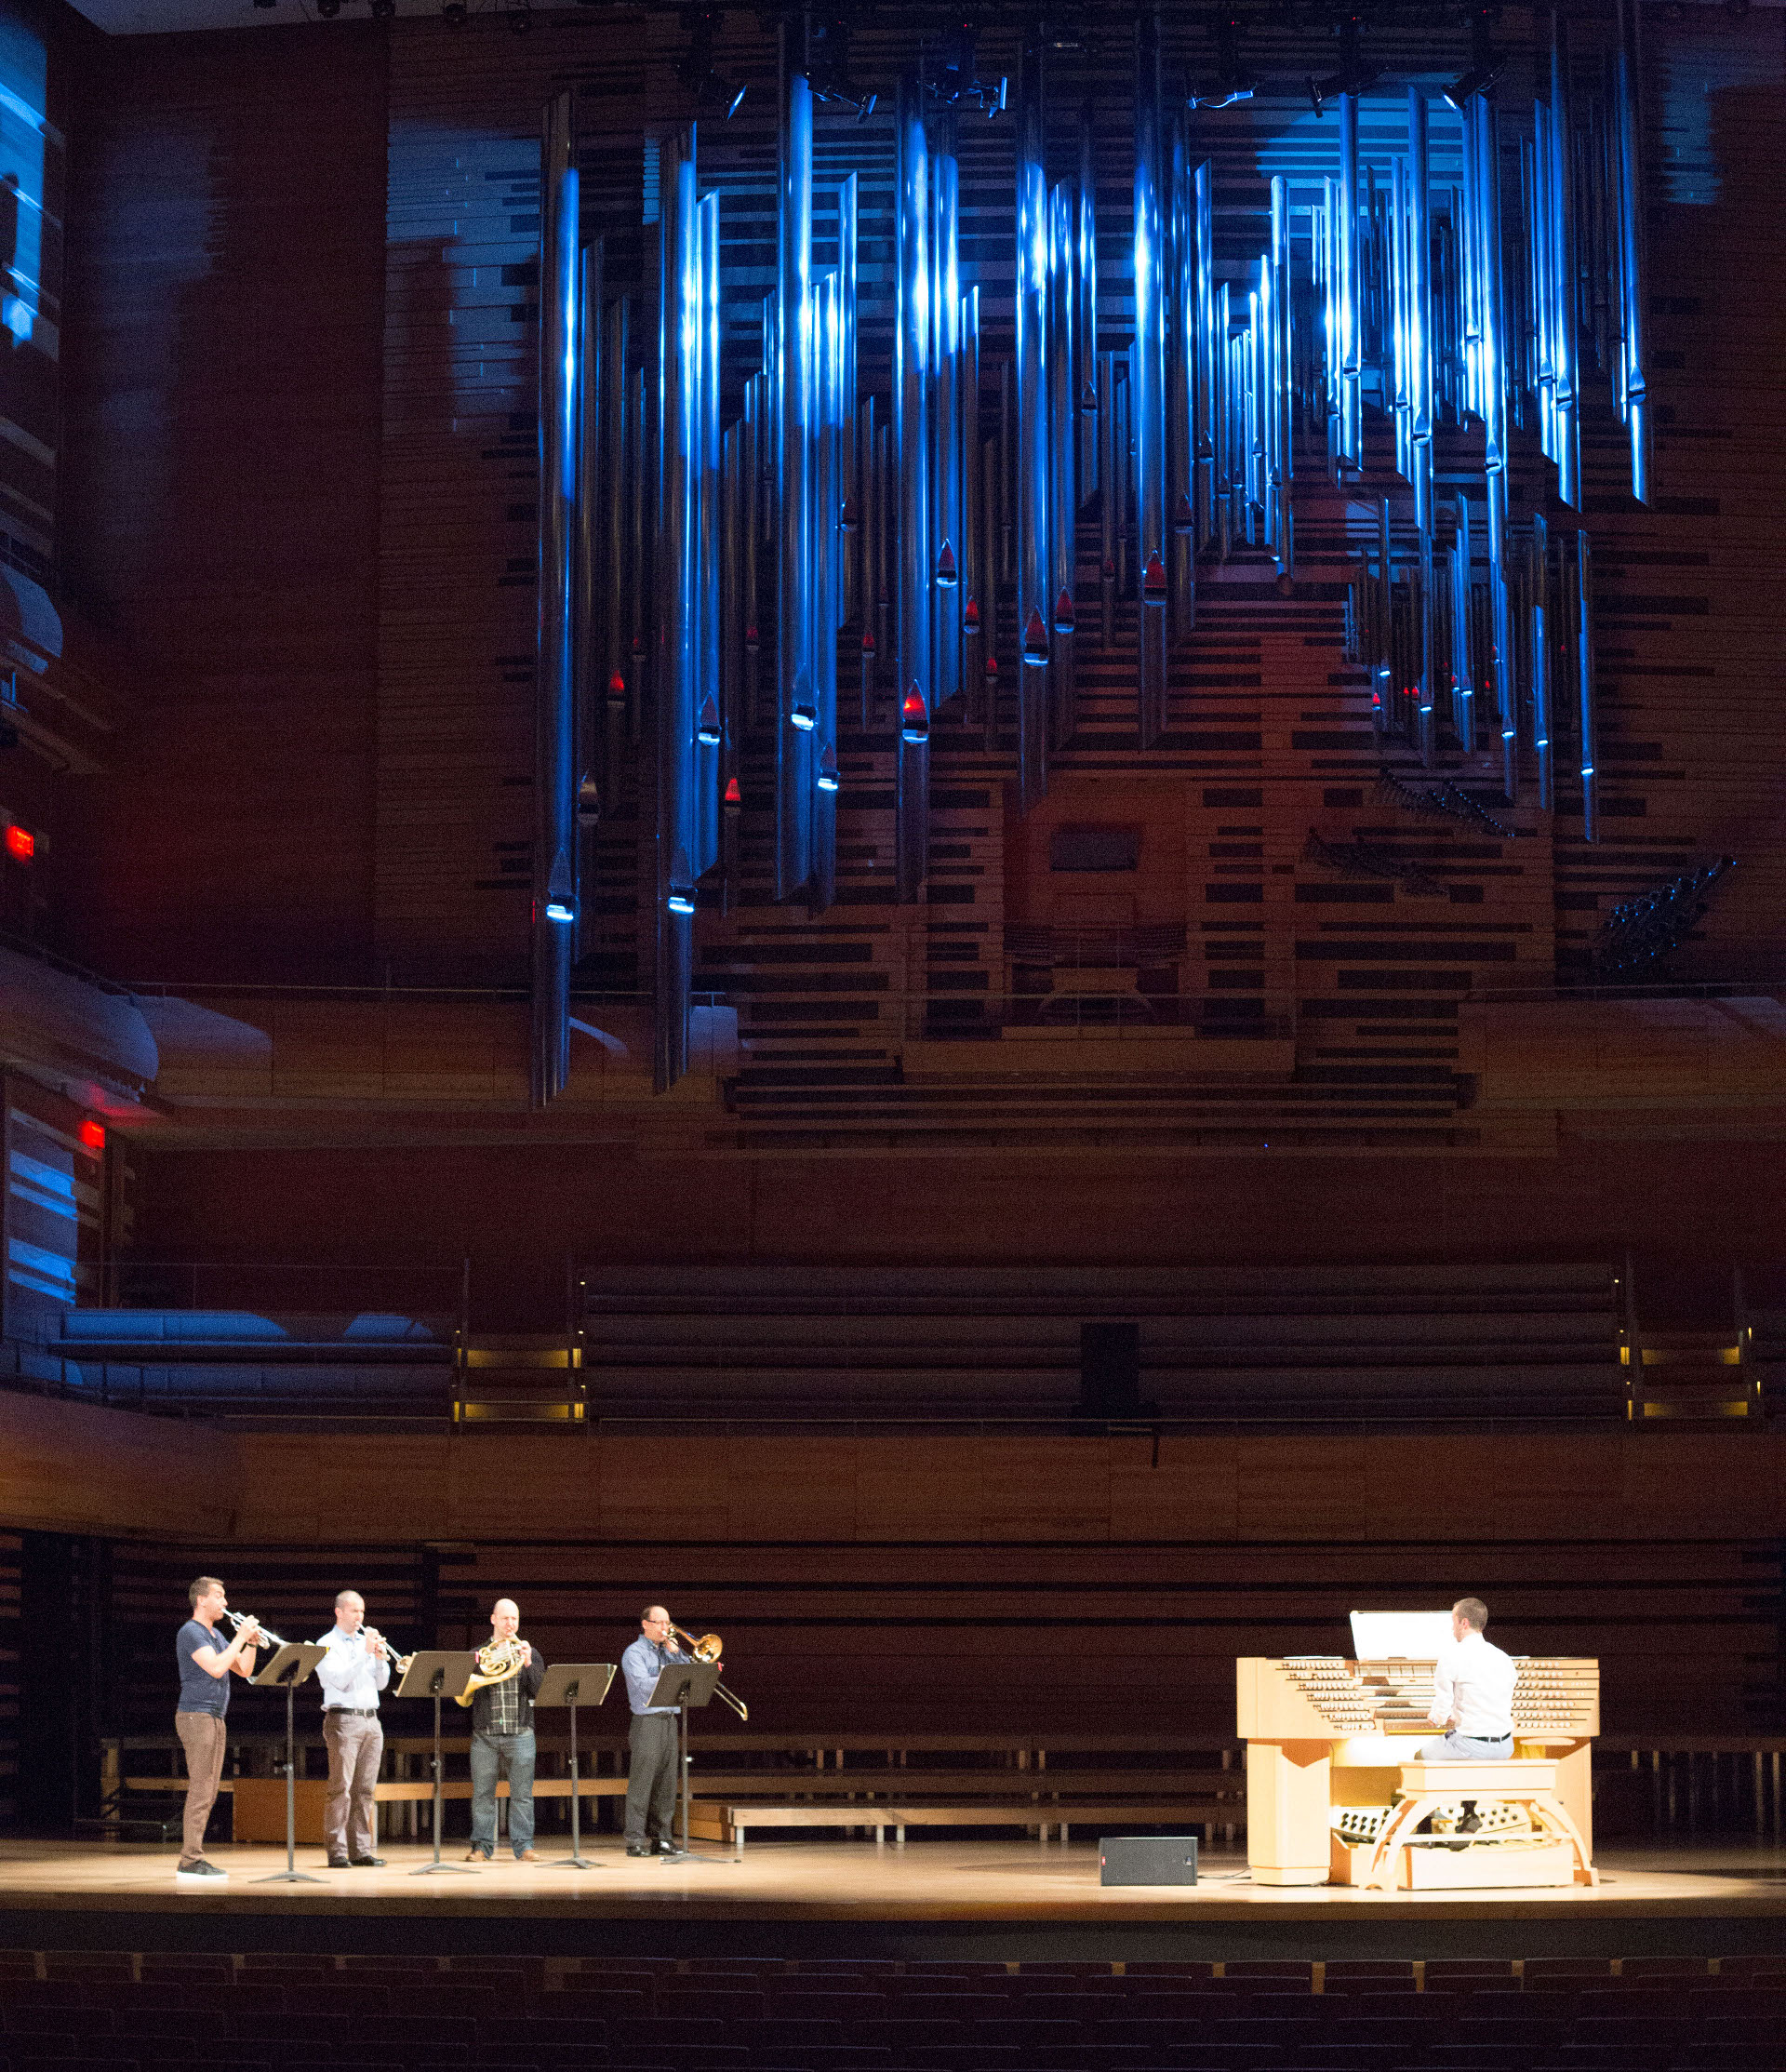
\includegraphics[width=\linewidth]{DressRehersal.jpg}
  \caption{The Pierre B\'{e}ique Organ in the OSM concert hall during
    a rehearsal on May 15th, 2015. Approximately 97\% of the organs'
    6489 pipes are out of sight behind the woodwork. Photo credit: Ben
    Bloomberg}
  \label{fig:le-corbusier-sketch}
\end{figure*}


%%% Local Variables:
%%% mode: latex
%%% TeX-master: "CharlesHolbrow_MAS_Thesis"
%%% End:

\clearpage
\chapter{Discussion and Analysis}
\label{ch:analysis}
In the previous chapters, we explore three new tools for creating and
processing music, their motivations, and implementations. The \refmod
in chapter \ref{ch:ref-mod}, proposes a new way to think about sound
in space. The \polytempic in chapter \ref{ch:polytempic} does the same
with musical time and meter. Chapters \ref{ch:hypercompressor} and
\ref{ch:experience} describe and implement a technique for modulating
music in in space with time as a reference. Each project project
builds on Iannis Xenakis' theory of \textit{stochastic music}. Each
project incorporates elements from other disciplines including
mathematics, computer science, acoustics, audio engineering and
mixing, sound reinforcement, multimedia production, and live
performance.

This final chapter discusses how each project succeeded, how each
project failed, and how future iterations can benefit from lessons
learned during the development process.

\section{Evaluation Criteria}
\label{sec:eval-criteria}
To evaluate a project of any kind, it is helpful to begin with a
purpose, and then determine the granularity and scope of the
evaluation.\cite{Saltzer2009} We might evaluate a music recording for
audio fidelity, for musical proficiency of the artist, for emotional
impact or resonance, for narrative, for technological inovation, for
creative vision, or for political and historical insight. This also
applies to the evaluation of technology.  We can evaluate the
suitability of a rack-mount analog to digital converter (ADC) for a
given purpose. A recording engineer may prefer the device impart a
favorable sound, while an acoustician may prefer that the device be
as neutral as possible. However, when evaluating an ADC or a music
recording, what we are most concerned with is the top level interface:
From most perspectives, we evaluate music by listening to it, and we
are not concerned which ADC was used to make the recording. When an
audio engineer, or acoustician evaluates an ADC, the device's
performance is more important than the exact layout of electronic
components inside the device.

Stochastic music theory is a \textit{vertical integration} of
mathematics, the physics of sound, psychoacoustics, and music. The
theory of stochastic music begins with the lowest level components of
sound, and ends with a creative musical product. What is a reasonable
perspective from which to evaluate stochastic music? From the
perspective of a listening, or performing the music? From the
perspective of a historian, evaluating the environment that led to the
composition, or studying the impact on music afterwords?  Should we try
to make sense of the entire technology stack, or try to evaluate every
layer of abstraction individually?

Somehow, between the low-level elements of sound and a musical
composition or performance, we transition from what is numerically
quantifiable to what we can only attempt to describe. The impossible
challenge of quantifying the unquantifiable is exactly what makes
music technology and audio engineering so alluring.

\TODO{What approach did I use?} I avoid comparative analysis, or
evaluation based on any kind of rubrik. 

%  Does the unit have an appropriate number and type of audio outputs suit
% our needs (such as TRS, XLR, and USB)? Does it perform reliably? Does
% it have a neutral or favorable impact on the sound? The results of our
% evaluation will depend on our purpose. If the purpose of the device is
% for playback of audio in a live performance context, the best choice
% will be different than if we want to use the unit for mixing in a
% recording studio.

\section{\refmod}
This project provides a single abstract interface that approaches
composition of space (architecture) and the composition of music at
the same time. The forms that it makes are familiar from the ruled
surfaces seen in Xenakis compositions, and early sketches of the
Philips Pavilion. In musical mode, we can think of the x and y axes
representing time and pitch. In architectural mode the canvas might
represent the floor plan of spaces we are designing.

While it is interesting to switch our perspective between the two
modes, there is not a clear connection from one to the other. A
carefully designed surface or reflection in one mode would be quite
arbitrary in the other mode. The reason that the interface is capable
of working in both modes is because it is so minimalist, that it does
not commit to one or the other. This is not a complete failing: The
tool was really designed to be a brainstorming aid at the very
beginning of the design process. It can be much simpler and quicker to
use that proper architectural software, as a means of creating
abstract shapes, similar to sketching on paper, before turning to
specialized software for more detailed design.

\paragraph{Curves, Constraints, and Simplicity} Despite the
shortcomings in this project, the parts that worked well and make a
good starting point for future iterations. There's something
intangible, but simple and \textit{fun} about the user
interface. There is only one input action; dragging a control
point. It is immediately clear what each control point does when it is
moved. It is easy to not even notice that there are five different
types of control points and each has slightly different behavior. It
is very intuitive to adjust a reflection surface such that the red
beams \textit{focus} on a certain point, and then re-adjust a
reflection surface so that they diverge chaotically. There is
something fascinating about how the simple movements intuitively
produce simultaneously coordinated or chaotic results. The response
might be described as \textit{stochastic}!

The red ``sound lines'' have three degrees of freedom: Position,
direction, and length. We can point the rays in any direction we like,
but, their movement is somewhat constrained.  The projection angle is
locked to 30 degrees, and the number of beams is always 8. Most of the
flexibility from the interface comes from the reflective surfaces.

It is easier to draw a curving reflective surface than a strait
one. If you make a special effort, it is possible to make one of the
surfaces straight, but just like drawing a line on a paper with a pen,
curved surfaces come more naturally. However, the curves in the \refmod do not
come naturally because they are following an input gesture like most
``drawing'' interfaces, but because of the simple mathematics in the
of the Bezier curves. Similarly, if we consider the red lines to be
notes on a time/pitch axis, the default interpretation is stochastic
glissandi rather than static pitches. Most musical software assumes
static pitches by default, and most architectural software assumes
strait lines by default.

\paragraph{Next Steps}
The obvious next steps, for this project, are correcting the
shortcomings described above. It could be made to work in three
dimensions, and model precise propagation of sound, rather than a very
simplified abstraction: It could become a proper acoustical
simulator. Another possibility is playing the sound is turning it into
a musical instrument where we can hear the stochastic glissandi in
realtime. These options are not necessarily mutually exclusive, but as
the interface becomes tailored to a more specific application, our
ability to think about the content as abstract representations also
breaks down. The ideal of software that is equally well equipped to
compose music and to imagine architectural spaces is probably
unrealistic. The beauty of the abstract representation of music
composition, is that \textit{any} visual representation of music is
quite abstract.

However, the direction I would like to take this in is not 

% Describe where I want to take this.
\section{\polytempic}
This chapter presents a very pure and elegant solution to a very
complex problem. But is it important? Is it not enough to just change
tempo with any of the other techniques presented in section
\ref{sec:background-polytempi}? If a performer cannot play precise tempo
curves anyway, what is this actually for?

Western polytempic music as defined in this chapter has existed for
only slightly over than one century, and there is certainly room for
new explorations. The oldest example in of western polytempic music is
in by Charles Ives in his 1906 piece, \textit{Central Park in the
  Dark}.\cite{Greschak2003} In the piece, the string section
represents nighttime darkness, while the rest of the orchestra
represents the sounds of central park at night. Beginning at measure
64, Ives leaves a note in the score, describing how the orchestra
accelerates, while the string section plays a constant tempo:
\begin{quotation}
  From measure 64 on, until the rest of the orchestra has played
  measure 118, the relation of the string orchestra's measures to
  those of the other instruments need not and cannot be written down
  exactly, as the gradual accelerando of all but the strings cannot be
  played in precisely the same tempi each time.
\end{quotation}
Ives acknowledges that there is no notation to describe the effect
that he wants, and that musicians are not capable of playing the
transition in a precise way. In this example, it is not important that
the that the simultaneous tempi have a precise rhythmic
relationship. Ives' use of paralel tempi is a graceful one. He
achieves a particular effect without requiring the musicians to do
something so unnatural as accelerate and decelerate relative to each
other, and then resynchronize at certain points. 

All polytempic compositions must grapple with the issue of
syncronicity, and most are less elegant than \textit{Central Park in
  the Dark}. Stockhausen's \textit{Gruppen} uses polytempi very
aggressively, going to great lengths to ensure that the three
orchestras are rhythmically synchronized and desynchronize in just the
right way.  If Stockhausen had been able to control the syncronicity
of the tempo precisely, it seems likely that he would have wanted
to try it. At least he would have been interested in experimenting with
\polytempic in other compositions.

\paragraph{Next Steps} Some music (and perhaps stochastic music in
particular) may be more interesting or influential from a theoretical
perspective than for the music itself in isolation. It could be that
the possibilities unlocked through the equations derived in
\autoref{ch:polytempic} are not different enough from the
approximations used by Nancarrow and Cage. Or that it is unrealistic
to direct performers to play them accurately enough to perceive the
difference.

However it is surprising that current digital tools for composition do
not let us even \emph{try} \polytempic. If we want to hear what tempo
transitions like the ones describe here sound like using digital
technology, there is no software that lets us do so, and we are still
forced to approximate. 

Audio programming languages like Max and SuperCollider let us code
formulaic tempi into our compositions, but equations like the ones
derived here are still required. I could not find any any mathematical
technique that lets us create tempo accelerations that fit the
constraints described in \autoref{ch:polytempic}, or any musical
example that proposed to have found another solution.

For simple cases, approximation is probably acceptable. If a musician
is incapable of playing the part, we are also likely incapable of
hearing the subtleties that distinguish an approximation from a
perfect performance. However, if we want lage collections of
simultaneous polytempi, like the ones shown in
figures~\ref{fig:polytempic-transition}
and~\ref{fig:polytempic-transition-3}, the approximations possible
with transcriptions, or the approximations of an unassisted human
performers are not precise enough.

\paragraph{Stochastic Theory} The study of \polytempic reveals what is
probably the greatest strength of stochastic music theory. A vertical
integration of the theory of sound and music lets us experience music
from a different perspective, and discover missed opportunities along the
way. 

\section{\thesis}
The design and development of the hypercompressor happened in parallel
with pre-production for \textit{De L'Exp\'{e}rience}. Often design
decisions were based on the factors involved with this one project,
not the most general case. The resulting project leave significant
design questions surrounding ambisonic dynamic range compression
unanswered.  For example: What it the best way to detect and attenuate
a region on our surround spere that is an unusual or elongated shape?
Should the compressor attempt to attenuate the narrow region only?
Should we the center of the region be attenuated by the same amount as
the very edge? The decision to make the surround compressor warp the
surround image in addition to attenuating regions that exceed the
threshold was also chosen because it suited the use case.
\begin{itemize}
\item We could simply warp all sounds away from a region that exceeds
  the compression threshold without attenuating them at all. However,
  doing so would increase the perceived level of the sound coming from
  the opposite direction. We also run the risk of creating the sonic
  ping-poing of sound arbitrarily panning around us just for the sake
  of the excitement, but not serving any larger artistic goal. 
\item If we simply attenuate a region that exceeds the threshold, we
  are not taking advantage of the opportunities provided to us by
  surround sound in the first place. In side-chain mode, we risk
  hiding a compressed sound completely when we could simple warp that
  region of the surround field to a location where it can be heard
  more clearly.
\end{itemize}
The current implementation also does not handle the case when two
separate regions of the surround field both exceed the threshold. What
are the ideal results? 

Another use case that is handled is that
when two sounds at a right angle (for example, one sound straight in
front of the listener, and one sound 90\degree{} to the right) both
exceed the threshold. The current implementation behaves
\paragraph{Stochos}

\paragraph{\textit{De L'Exp\'{e}rience}}
The main goal, of using the Hypercompressor was to blend the
electronic textures with the sound of the Pierre B\'{e}ique organ in
Tod Machover's composition . The chosen approach as to give the
electronics a sense of motion that the organ, (who's sound is awe
inspiring, but also somewhat static) cannot produce; thus the
electronics can be heard moving \emph{around} the sound of the organ,
rather than being required to compete with the sound of the organ.
The first attempt at this goal, however was not a success.

The electronics were mixed to occupy as much of the surround sound
sphere as possible, filling the entire room with sound.  My original
idea was to spatially separate the organ and electronics by connecting
them to the Hypercompressor in side-chain mode.  When the organ was
playing it would \emph{push} the sound of the electronics to the back
of the room, making it easier to hear both timbres without either
masking the other.  During the \textit{De L'Exp\'{e}rience} rehearsal,
this was the first approach I tried, but the resulting surround
texture had a different problem: The sound of the organ and the sound
of the electronics were \emph{too} separate. They did not blend with
each other in space, but existed as two clearly distinct sources. The
final solution (described in \autoref{ch:hypercompressor}) was the
result of the unsatisfactory results from my first attempt. While it
did not end up working the way I anticipated, I consider the
Hypercompressor to have aided the blending of the organ and
electronics rather well. However, the beautiful blend of electronic
and acoustic sounds that we achieved would have been possible without
many other contributing factors, such as the expert composition of the
electronic textures.

\paragraph{Next Steps}

\section{overall}
It would appear that the main challenge with stochastic composition,
or vertical integration, or that of scope. 

Having mixed a bunch of stuff, for different contexts, the different
panning strategies in discrete channel, ambisonics, don't are not
better or worse. Stockhausen didn't really didn't need anything other than
discrete channel panning for Gesang. In fact the piece holds up very
well in stereo. I do think that there is a difference between actual
surround and 5.1, the latter resembling dual stereo more than actual
surround. 

% welp, not sure how well it actually
% worked. And I don't expect electronic instrument to ever replace
% acoustic instruments, although they may eventually equal them in
% expressivity. Initially thought it would work backwards

%%% Local Variables:
%%% mode: latex
%%% TeX-master: "CharlesHolbrow_MAS_Thesis"
%%% End:


\backmatter
\chapter*{Acknowledgements}
\label{ch:acknowledgements}

\begin{fullwidth}
Thanks to Tod Machover, for your continuous support and encouragement,
for sharing your process, and for help and support integrating \thesis
into \textit{Of Experience}.

Thanks to James Andy Moorer and Joe Paradiso for support, guidance and
mentorship.\TODO{verify spelling}

Thanks to professor Alex Case for the most inspiring my love for
music, audio engineering, and illuminating the magical subtleties of
dynamic range compression.

Thanks to Wonshik Choi and Niyom Lue for your infinite patience,
guidance, and for welcoming me to MIT in 2008. Only you could have
taught a music major to enjoy linux, DSP, and spectroscopy.

Thanks to Shawn Drost for directly and indirectly giving me confidence
as a software developer.

Thanks to my UMass Lowell Piano teachers for taking chance with me,
and putting up with me for four years. Anthony Mele, Elizabeth
Skavish, Bonnie Anderson, and Thomas Stumpf - You believed in me
before I did. I'm probably the only student ever who was lucky enough
to study with all four of you. :P

Thanks to Gene Atwood for being considerate of everyone, and showing
me how important that is -- And for screaming in to a microphone when
I needed some screams.

Thanks to Ben Bloomberg for being my peer and my mentor at the same
time. Thanks for bringing me into the Opera group in 2008 and bringing
me back in 2014. Thanks to Bryn Bliska, for proposing polytempic
modulation, and sharing letting me work out the maths. Thanks to
Rebecca Kleinberger and Akito Van Troyer for your unending support and
encouragement. 

Thanks to Helen Corless for being amazing supportive even when I am in
the absolute pits of grad student existence. Thank you for always
reminding me what music is really about, and for challenging me like
no one else can.

Thanks to my grandparents for leading by example, and teaching
kindness and dedication, and for endless support in education.

Thanks to Hilary, Giles, and Felicity for always inspiring me with
kindness, honesty, and wisdom. 

And thanks to my parents, Gwen and Mark for forcing me to get an
education before I was wise enough to know I wanted one. Thank you for
all your love and support in everything ever I have ever done.
\end{fullwidth}
%%% Local Variables:
%%% mode: latex
%%% TeX-master: t
%%% End:


\bibliography{library}
\bibliographystyle{plainnat}

\end{document}


%%% Local Variables:
%%% mode: latex
%%% TeX-master: t
%%% End:
